%%%%%%%%%%%%%%%%%%%%%%%%%%%%%%%%%%%%%%%%%%%%%%%%%%%%%%%%%%%%%%%%%%%%%%%%
% Uni Duesseldorf
% Lehrstuhl fuer Datenbanken und Informationssysteme
% Vorlage fuer Bachelor-/Masterarbeiten
% Optimiert fuer den Original-Latex-Kompiler LATEX.EXE (LaTeX=>PS=>PDF)
%%%%%%%%%%%%%%%%%%%%%%%%%%%%%%%%%%%%%%%%%%%%%%%%%%%%%%%%%%%%%%%%%%%%%%%%
% Ueberarbeitung für pdflatex (LaTeX=>PDF)
%%%%%%%%%%%%%%%%%%%%%%%%%%%%%%%%%%%%%%%%%%%%%%%%%%%%%%%%%%%%%%%%%%%%%%%%
% Vorlage Changelog:
% 10.09.2015 (Matthias Liebeck): Nummerierung des Inhaltsverzeichnis nun römisch, Beispiel für einen Anhang eingebaut, \raggedbottom hinter sections eingefügt
%%%%%%%%%%%%%%%%%%%%%%%%%%%%%%%%%%%%%%%%%%%%%%%%%%%%%%%%%%%%%%%%%%%%%%%%
%%%% BEGINN EINSTELLUNG FUER DIE ARBEIT. UNBEDINGT ERFORDERLICH! %%%%%%%
%%%%%%%%%%%%%%%%%%%%%%%%%%%%%%%%%%%%%%%%%%%%%%%%%%%%%%%%%%%%%%%%%%%%%%%%
% Geben Sie Ihren Namen hier an:
\newcommand{\bearbeiter}{Johannes Thiel}

% Geben Sie hier den Titel Ihrer Arbeit an:
\newcommand{\titel}{Mustererkennug und Live-Analyse von Videos zu Kartenspielen}

% Geben Sie das Datum des Beginns und Ende der Bachelorarbeit ein:
\newcommand{\beginndatum}{28.~M\"arz~2017}
\newcommand{\abgabedatum}{27.~Juni~2017}

% Geben Sie die Namen des Erst- und Zweitgutachters an:
\newcommand{\erstgutachter}{Prof. Dr.~Michael Leuschel}
\newcommand{\zweitgutachter}{Dr.~Katja Hansen}

% Falls Sie die Arbeit zweiseitig ausdrucken wollen,
% benutzen Sie die folgende Zeile mit
% \AN fuer zweiseitigen Druck
% \AUS fuer einseitigen Druck
\newcommand{\zweiseitig}{\AN}

% Falls die Arbeit in englischer Sprache verfasst 
% werden soll, dann benutzen Sie die folgende Zeile mit
% englisch fuer englische Sprache
% deutsch fuer deutsche Sprache
\newcommand{\sprache}{deutsch}

% Hier wird eingestellt, ob es sich bei der Arbeit um eine Bachelor- 
% oder Masterarbeit handelt (unpassendes auskommentieren!):
\newcommand{\arbeit}{Bachelorarbeit}
%~ \newcommand{\arbeit}{Masterarbeit}

%%%%%%%%%%%%%%%%%%%%%%%%%%%%%%%%%%%%%%%%%%%%%%%%%%%%%%%%%%%%%%%%%%%%%%%%
%%%% ENDE EINSTELLUNGEN %%%%%%%%%%%%%%%%%%%%%%%%%%%%%%%%%%%%%%%%%%%%%%%%
%%%%%%%%%%%%%%%%%%%%%%%%%%%%%%%%%%%%%%%%%%%%%%%%%%%%%%%%%%%%%%%%%%%%%%%%

% Die folgende Zeile NICHT EDITIEREN oder loeschen


%%%%%%%%%%%%%%%%%%%%%%%%%%%%%%%%%%%%%%%%%%%%%%%%%%%%%%%%%%%
% Obere Titelmakros. Editieren Sie diese Datei nur, wenn
% Sie sich ABSOLUT sicher sind, was Sie da tun!!!
% (Z.B. zum Abaendern der BA-Vorlage in eine MA-Vorlage)
% Uni Duesseldorf
% Lehrstuhl fuer Datenbanken und Informationssysteme
% Version 2.2 - 2.3.2010
%%%%%%%%%%%%%%%%%%%%%%%%%%%%%%%%%%%%%%%%%%%%%%%%%%%%%%%%%%%
\newcommand{\AN}{twoside}
\newcommand{\AUS}{}
%\newcommand{\englisch}{}
%\newcommand{\deutsch}{\usepackage[german]{babel}}

%% Die folgenden auskommentierten Optionen dienen der automatischen
%% Erkennung des Latex-Kompilers und dem Setzen der davon abhängigen
%% Einstellungen. Bei Problem z.B. mit dem Einbinden von verschiedenen
%% Grafiktypen bei Verwendung von PdfLatex oder Latex, einfach die
%% verschiedenen \usepackage(s) ausprobieren. (Mit diesen Einstellungen
%% funktionierte diese Vorlage bei der Verwenundg von latex.exe als
%% Kompiler bei den meisten Studierenden.)

%\newif\ifpdf \ifx\pdfoutput\undefined
%\pdffalse % we are not running pdflatex
%\else
%\pdfoutput=1 % we are running pdflatex
%\pdfcompresslevel=9 % compression level for text and image;
%\pdftrue \fi

\documentclass[11pt,a4paper, \zweiseitig]{article}



%\usepackage[iso]{umlaute}
\usepackage[utf8x]{inputenc}
\usepackage{palatino} % palatino Schriftart
%\usepackage{makeidx} % um ein Index zu erstellen
\usepackage[nottoc]{tocbibind}
\usepackage[T1]{fontenc} %fuer richtige Trennung bei Umlauten
\usepackage{fancybox} % fuer die Rahmen
\usepackage{shortvrb}
\usepackage{ifthen}
\ifthenelse{\equal{\sprache}{deutsch}}{\usepackage[ngerman]{babel}}{}

\usepackage{a4wide} % ganze A4 Weite verwenden

%\ifpdf
%\usepackage[pdftex,xdvi]{graphicx}
%\usepackage{thumbpdf} %thumbs fuer Pdf
%\usepackage[pdfstartview=FitV]{hyperref} %anklickbares Inhaltsverzeichnis
%\else
%\usepackage[dvips,xdvi]{graphicx}
\usepackage{graphicx}
\usepackage{hyperref} %anklickbares Inhaltsverzeichnis
%\fi

%%%%%%%%%%%%%%%%%%%%%%% Massangaben fuer die Arbeit %%%%%%%%%%%%%%%
\setlength{\textwidth}{15cm}

\setlength{\oddsidemargin}{35mm}
\setlength{\evensidemargin}{25mm}

\addtolength{\oddsidemargin}{-1in}
\addtolength{\evensidemargin}{-1in}

\usepackage{subcaption}
\usepackage{booktabs} % Horizontal rules in tables
\usepackage{amsmath}
\usepackage{amssymb}
\DeclareMathOperator{\atantwo}{atan2}
\DeclareMathOperator*{\argmax}{arg\,max}
%\makeindex

\begin{document}

%\setcounter{secnumdepth}{4} %Nummerieren bis in die 4. Ebene
%\setcounter{tocdepth}{4} %Inhaltsverzeichnis bis zur 4. Ebene

\pagestyle{headings}

\sloppy % LaTeX ist dann nicht so streng mit der Silbentrennung
%~ \MakeShortVerb{\§}

\parindent0mm
\parskip0.5em


{
\textwidth170mm 
\oddsidemargin30mm 
\evensidemargin30mm 
\addtolength{\oddsidemargin}{-1in}
\addtolength{\evensidemargin}{-1in}

\parskip0pt plus2pt

% Die Raender muessen eventuell fuer jeden Drucker individuell eingestellt
% werden. Dazu sind die Werte fuer die Abstaende `\oben' und `\links' zu
% aendern, die von mir auf jeweils 0mm eingestellt wurden.

%\newlength{\links} \setlength{\links}{10mm}  % hier abzuaendern
%\addtolength{\oddsidemargin}{\links}
%\addtolength{\evensidemargin}{\links}

\begin{titlepage}
\vspace*{-1.5cm}
  \raisebox{17mm}{
    \begin{minipage}[t]{70mm}
      \begin{center}
        %\selectlanguage{german}
        {\Large INSTITUT FÜR INFORMATIK\\}
        {\normalsize
          Datenbanken und Informationssysteme\\
        }
        \vspace{3mm}
        {\small Universitätsstr. 1 \hspace{5ex} D--40225 Düsseldorf\\}
     \end{center}
    \end{minipage}
  }
  \hfill
  
\includegraphics[width=130pt]{bilder/HHU_Logo}
  \vspace{14em}

% Titel
  \begin{center}
      	\baselineskip=55pt
    	\textbf{\huge \titel}
  	 	\baselineskip=0 pt
   \end{center}

  %\vspace{7em}

\vfill

% Autor
  \begin{center}
    \textbf{\Large
      \bearbeiter
    }
  \end{center}

  \vspace{35mm}
 
% Prüfungsordnungs-Angaben
  \begin{center}
    %\selectlanguage{german}
    
%%%%%%%%%%%%%%%%%%%%%%%%%%%%%%%%%%%%%%%%%%%%%%%%%%%%%%%%%%%%%%%%%%%%%%%%%
% Ja, richtig, hier kann die BA-Vorlage zur MA-Vorlage gemacht werden...
% (nicht mehr nötig!)
%%%%%%%%%%%%%%%%%%%%%%%%%%%%%%%%%%%%%%%%%%%%%%%%%%%%%%%%%%%%%%%%%%%%%%%%%
    {\Large \arbeit}

    \vspace{2em}

    \begin{tabular}[t]{ll}
      Beginn der Arbeit:& \beginndatum \\
      Abgabe der Arbeit:& \abgabedatum \\
      Gutachter:         & \erstgutachter \\
                         & \zweitgutachter \\
    \end{tabular}
  \end{center}

\end{titlepage}

}

%%%%%%%%%%%%%%%%%%%%%%%%%%%%%%%%%%%%%%%%%%%%%%%%%%%%%%%%%%%%%%%%%%%%%
\clearpage
\begin{titlepage}
  ~                % eine leere Seite hinter dem Deckblatt
\end{titlepage}
%%%%%%%%%%%%%%%%%%%%%%%%%%%%%%%%%%%%%%%%%%%%%%%%%%%%%%%%%%%%%%%%%%%%%
\clearpage
\begin{titlepage}
\vspace*{\fill}

\section*{Erklärung}

%%%%%%%%%%%%%%%%%%%%%%%%%%%%%%%%%%%%%%%%%%%%%%%%%%%%%%%%%%%
% Und hier ebenfalls ggf. BA durch MA ersetzen...
% (Auch nicht mehr nötig!)
%%%%%%%%%%%%%%%%%%%%%%%%%%%%%%%%%%%%%%%%%%%%%%%%%%%%%%%%%%%

Hiermit versichere ich, dass ich diese \arbeit~
selbstständig verfasst habe. Ich habe dazu keine anderen als die
angegebenen Quellen und Hilfsmittel verwendet.

\vspace{25 mm}

\begin{tabular}{lc}
Düsseldorf, den \abgabedatum \hspace*{2cm} & \underline{\hspace{6cm}}\\
& \bearbeiter
\end{tabular}

\vspace*{\fill}
\end{titlepage}

%%%%%%%%%%%%%%%%%%%%%%%%%%%%%%%%%%%%%%%%%%%%%%%%%%%%%%%%%%%%%%%%%%%%%
% Leerseite bei zweiseitigem Druck
%%%%%%%%%%%%%%%%%%%%%%%%%%%%%%%%%%%%%%%%%%%%%%%%%%%%%%%%%%%%%%%%%%%%%

\ifthenelse{\equal{\zweiseitig}{twoside}}{\clearpage\begin{titlepage}
~\end{titlepage}}{}

%%%%%%%%%%%%%%%%%%%%%%%%%%%%%%%%%%%%%%%%%%%%%%%%%%%%%%%%%%%%%%%%%%%%%
\clearpage
\begin{titlepage}

%%% Die folgende Zeile nicht ändern!
\section*{\ifthenelse{\equal{\sprache}{deutsch}}{Zusammenfassung}{Abstract}}
%%% Zusammenfassung:
Ziel der vorliegenden Arbeit ist es eine Grundlage für eine Anwendung zu schaffen, die Karten des Spiels ''Magic The Gathering'' in Echtzeitvideos finden und erkennen kann.

Hierfür werden drei verschiedene Verfahren ''Scale-Invariant Feature Transform'' (SIFT) \footnote{\cite{Lowe2004}}, ''Speeded Up Robust Features'' \footnote{\cite{Bay:2008:SRF:1370312.1370556}} (SURF) und ''Oriented FAST and Rotated BRIEF'' \footnote{\cite{Rublee:2011:OEA:2355573.2356268}} (ORB)  betrachtet, die Bildmerkmale erzeugen. Mit diesen wird ein Klassifikator erstellt, der Bildausschnitten von Karten aus Videobildern der Ursprungskarte zuordnen kann.
Um die Erkennungsrate des Klassifikators in Verbindung mit den einzelnen Verfahren zu überprüfen, wird händisch ein Testdatensatz erstellt. Mit diesem wird sowohl die Erkennungsrate als auch die Geschwindigkeit der Vefahren geprüft.
Die drei Verfahren kommen auf eine Erkennungsrate von 99.67\% (SIFT), 98.33\% (SURF) und 99.33\% (ORB).
Jedoch sind SIFT und SURF zu langsam, um eine Erkennung in Echzeit zu gewährleisten.
Es wird aufgezeit, dass SIFT in kleinen Bildern eine Tendenz hat, viele Bildmerkmale an Kanten zu finden.
Es wird zudem ein Verfahren entwickelt, mit dem Karten in Videobildern lokalisiert werden können.  In Kombination mit dem Klassifikator können so Karten automatisch in Videos gefunden und klassifiziert werden.
In einem Versuch, den Klassifikator durch mehr Trainingsdaten zu verbessern, werden Karten automatisch in Videos lokalisiert, klassifiziert und ausgeschnitten. Durch die Vergrößerung des Trainingsdatensatzes lässt sich eine geringe Verbesserung der Erkennungrate feststellen. Die Ergebnisse zeigen jedoch, dass mit mehr Videodaten die Erkennungsrate weiter verbessert werden kann.


%%%%%%%%%%%%%%%%%%%%%%%%%%%%%%%%%%%%%%%%%%%%%%%%
% Untere Titelmakros. Editieren Sie diese Datei nur, wenn Sie sich
% ABSOLUT sicher sind, was Sie da tun!!!
%%%%%%%%%%%%%%%%%%%%%%%%%%%%%%%%%%%%%%%%%%%%%%%
\vspace*{\fill}
\end{titlepage}

%%%%%%%%%%%%%%%%%%%%%%%%%%%%%%%%%%%%%%%%%%%%%%%%%%%%%%%%%%%%%%%%%%%%%
% Leerseite bei zweiseitigem Druck
%%%%%%%%%%%%%%%%%%%%%%%%%%%%%%%%%%%%%%%%%%%%%%%%%%%%%%%%%%%%%%%%%%%%%
\ifthenelse{\equal{\zweiseitig}{twoside}}
  {\clearpage\begin{titlepage}~\end{titlepage}}{}
%%%%%%%%%%%%%%%%%%%%%%%%%%%%%%%%%%%%%%%%%%%%%%%%%%%%%%%%%%%%%%%%%%%%%
\clearpage \setcounter{page}{1}
\pagenumbering{roman}
\setcounter{tocdepth}{2}
\tableofcontents

%\enlargethispage{\baselineskip}
\clearpage
%%%%%%%%%%%%%%%%%%%%%%%%%%%%%%%%%%%%%%%%%%%%%%%%%%%%%%%%%%%%%%%%%%%%%
% Leere Seite, falls Inhaltsverzeichnis mit ungerader Seitenzahl und 
% doppelseitiger Druck
%%%%%%%%%%%%%%%%%%%%%%%%%%%%%%%%%%%%%%%%%%%%%%%%%%%%%%%%%%%%%%%%%%%%%
\ifthenelse{ \( \equal{\zweiseitig}{twoside} \and \not \isodd{\value{page}} \)}
	{\pagebreak \thispagestyle{empty} \cleardoublepage}{\clearpage}



\pagenumbering{arabic}
\setcounter{page}{1}

%%%%%%%%%%%%%%%%%%%%%%%%%%%%%%%%%%%%%%%%%%%%%%%%%%%%%%%%%%%%%%%%%%%%%%%%
%%%% BEGINN TEXTTEIL %%%%%%%%%%%%%%%%%%%%%%%%%%%%%%%%%%%%%%%%%%%%%%%%%%%
%%%%%%%%%%%%%%%%%%%%%%%%%%%%%%%%%%%%%%%%%%%%%%%%%%%%%%%%%%%%%%%%%%%%%%%%

%%%%%%%%%%%%%%%%%%%%%%%%%%%%%%%%%%%%%%%%%%%%%%%%%%%%%%%%%%%%%%%%%%%%%%%%
% Text entweder direkt hier hinein schreiben oder, im Sinne der
% besseren Uebersichtlich- und Bearbeitbarkeit mittels \input die
% einzelnen Textteile hier einbinden.
%%%%%%%%%%%%%%%%%%%%%%%%%%%%%%%%%%%%%%%%%%%%%%%%%%%%%%%%%%%%%%%%%%%%%%%%

\section{Einleitung}\raggedbottom 

\subsection{Motivation}

Das Sammelkarten Spiel ''Magic The Gathering'' von Wizards of the Coast wird weltweit von etwa 20 Millionen  Spielern gespielt \footnote{\cite{GuardianMagicReport}}. 
Für das Spiel erscheinen regelmäßig neue Sätze an Karten. Spieler stellen aus der großen Auswahl an Karten eine eigene Auwahl zusammen, die als ''Deck'' bezeichnet wird, mit der sie gegen andere Spieler spielen.
Während des Spiels ziehen Spieler Karten von ihrem Deck und spielen diese strategisch in Zügen aus, mit dem Ziel, die ''Lebenspunkte'' des anderen Spielers von 20 auf 0 zu bringen.

Der Hersteller des Spieles betreibt eine große Turnierszene, in der Spieler aus aller Welt teilnehmen können.
In diesem Turniersystem sind über eine Millionen Spieler registriert und über 65000 \footnote{\cite[~p.7]{HasbroQ1Financial}}  nehmen in großen Turnieren mit mehreren tausend Spielern teil.
Diese großen Turniere werden im Internet live auf \url{twitch.tv/magic} übertragen. Besonders die Pro Tour, ein Event, zu dem die Spieler sich über andere Turniere qualifizieren müssen, lockt mehrere 10000 Zuschauer an \footnote{\cite{TwitchStat}}.

In diesen Liveübertragungen ist es nicht möglich, den Text auf Karten zu lesen (siehe Abbildung \ref{fig:screenshot}). Dieser ist jedoch für das Spiel sehr relevant, da, ohne den Text zu kennen, der Spielverlauf nicht nachvollzogen werden kann. 
Will ein Zuschauer verstehen, was im Spiel passiert, muss dieser die Karten anhand der Bildern auf ihnen identifizieren und auswendig wissen, was auf der jeweiligen Karte steht.

Dies ist besonders für neue Spieler und nach dem Erscheinen von neuen Karten ein Problem. 

Das Ziel dieser Arbeit soll es sein, ein Verfahren zu finden, welches automatisiert Karten in Videobildern finden und diese dann erkennen kann.
Dieses Verfahren soll als Grundlage für eine Anwendung dienen, welche automatisch Karten in einem Livevideo findet und den Kartentext bzw. ein Bild der Karte in lesbarer Qualität anzeigt.
Dadurch soll es neuen Spielern ermöglicht werden, Turniere zu verfolgen und den Spielverlauf zu verstehen.

\begin{figure}[h]
    \centering
		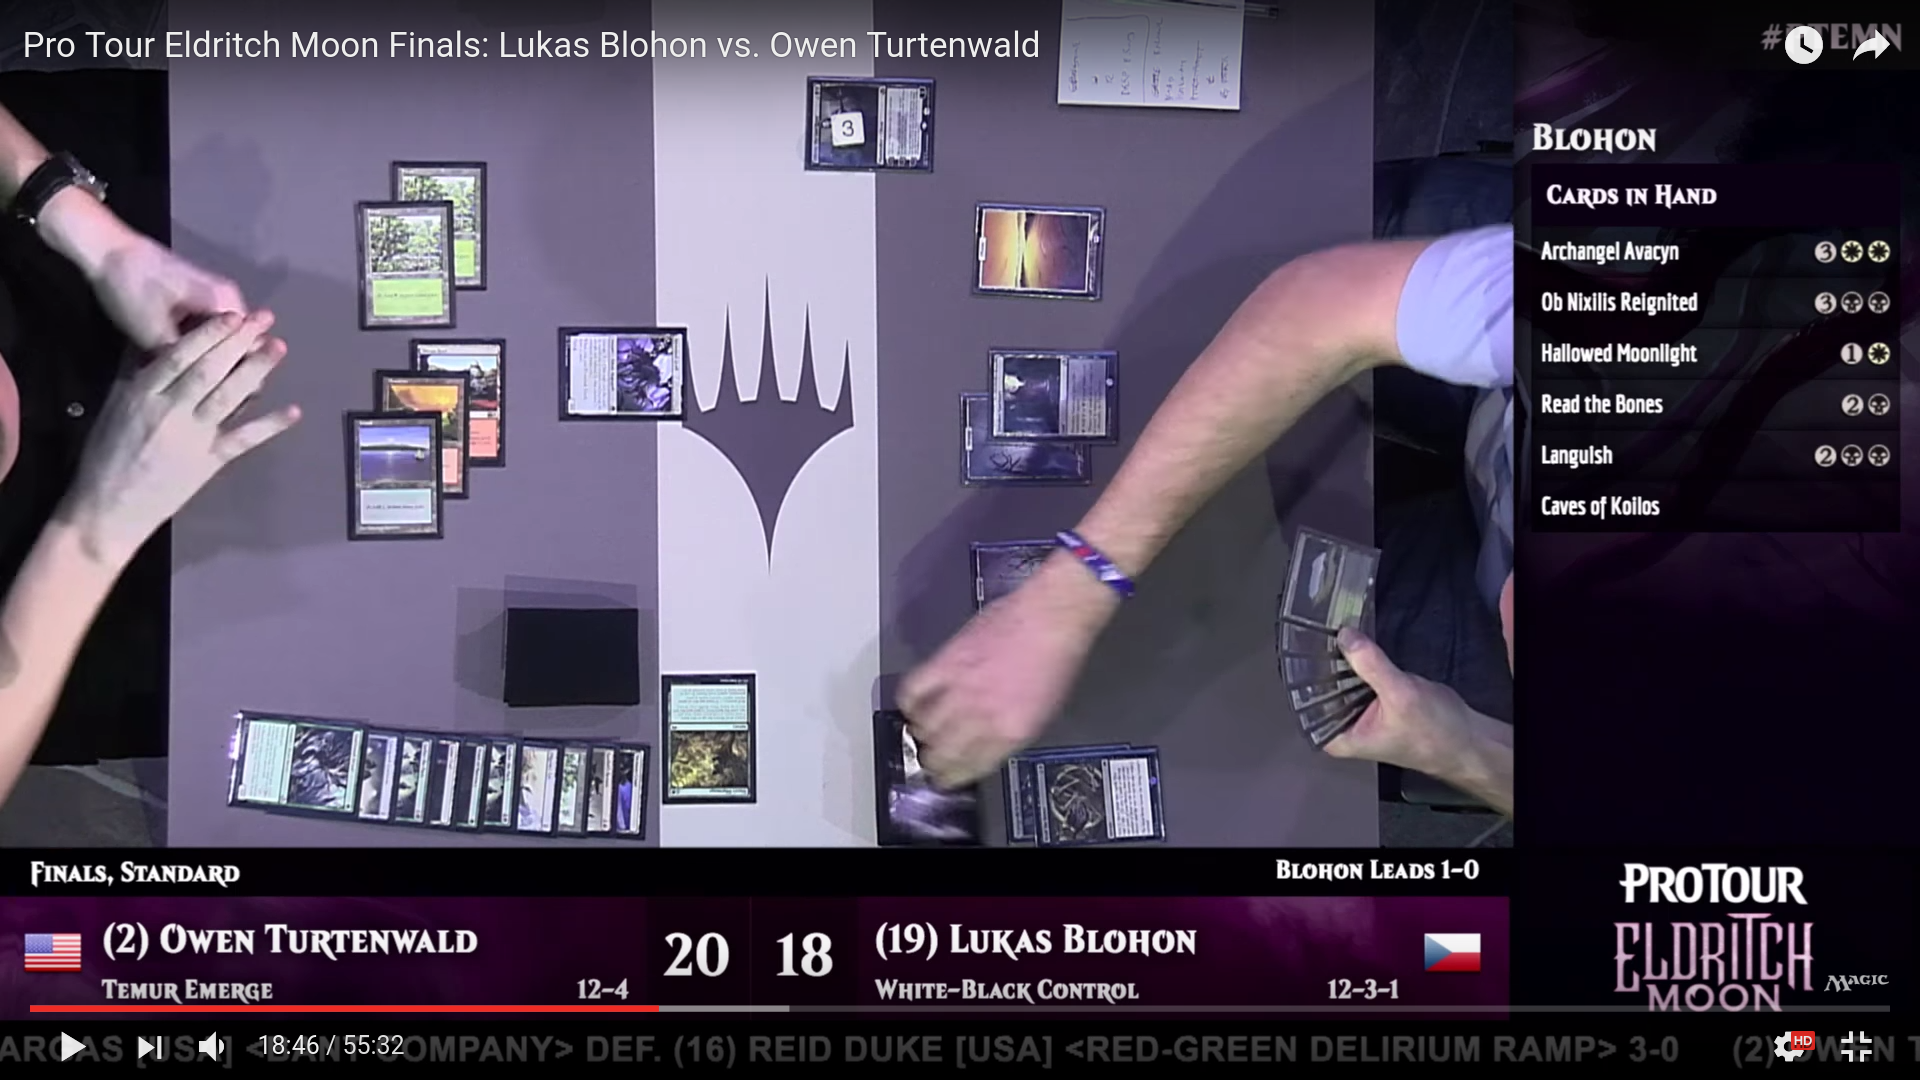
\includegraphics[scale=0.2]{bilder/screenshot.png}
    	\caption{Ein Bild aus den Videoaufnahmen.}
\label{fig:screenshot}
\end{figure}

\subsection{Aufbau} 

In dieser Arbeit werden zuerst grundlegende Methoden der Bildverarbeitung erläutert. Aufbauend auf diesen werden drei Verfahren betrachtet, die sogenannte Merkmale in einem Bild finden. Mit diesen Merkmalen können Objekte in verschiedenen Bildern wiedererkannt werden.


Es wird ein Klassifikator vorgestellt, der anhand der Merkmale, die diese Verfahren finden, Bilder von Karten klassifizieren kann.

Es wird ein Trainingsdatensatz erstellt, aus dem die Merkmale der einzelnen Karten berechnet werden. Dieser Trainingsdatensatz enthält Kartenbilder, die auf der offiziellen Seite des Herstellers zu finden sind.
 Zudem wird ein Testdatensatz erstellt. Dieser besteht aus Bildern von Karten, die aus Videos der Liveübertragung herausgeschnitten wurden. Zudem wird der Testdatensatz künstlich, mit häufig auftretenden Veränderungen, wie Rotation, erweitert. 

In einem Auswertungsteil wird die Erkennungsrate des Klassifikators mithilfe des Testdatensatzes analysiert.

Anschließend wird ein Verfahren vorgestellt, welches automatisch Karten in einem Videobild lokalisieren kann. In Verbindung mit dem Klassifikator können Karten so automatisch in einem Video gefunden und erkannt werden.
Dies wird genutzt, um den Trainingsdatensatz automatisch zu erweitern.
Es wird untersucht, ob diese Erweiterung zu einer besseren Erkennungsrate führt.


\section{Forschungsstand}\raggedbottom 
Karten in Videobildern zu erkennen stellt ein Problem der Objekterkennung dar.
Eine häufig verwendete Methode zur Objekterkennung sind Bildmerkmale.
Im Folgenden werden die Konzepte der Merkmalsdetektion (Feature Detection), Merkmalsbeschreibung (Feature Description) und des Merkmalsabgleiches (Feature Matching) beschrieben.
Desweiteren werden grundlegende Verfahren und Methoden der digitalen Bildverarbeitung erläutert, die in dieser Arbeit wichtig sind.

\subsection{Digitale Bildverarbeitung}

\subsubsection{Bildbeschreibung}

In der digitalen Bildverarbeitung gibt es mehrere Möglichkeiten, ein Bild zu beschreiben. Zwei häufig genutzte Bildbeschreibungen sind Rasterbilder und Vektorgrafiken \footnote{\cite[S. 15]{Burg06}}. In dieser Arbeit werden ausschließlich Rasterbilder betrachtet.

Ein Rasterbild ist eine zweidimensionale Matrix $I$ der Größe $n \times m$. Diese Größe wird im weiterem Auflösung genannt. Jedes Element dieser Matrix wird als Pixel bezeichnet.
Welche Informationen in jedem Pixel gespeichert sind, hängt von dem Typ des Bildes ab. Für diese Arbeit wichtig sind Grauwertbilder und Farbbilder.

Grauwertbilder speichern für jeden Pixel einen Wert zwischen 0 und 255. Dieser Wert beschreibt die Helligkeit bzw. Intensität an diesem Bildpunkt. Ein Wert von 0 steht hierbei für keine Helligkeit und ist somit schwarz. Ein Wert von 255 stellt eine maximale Helligkeit dar und ist somit weiß. 

Farbbilder speichern in jedem Pixel drei Komponenten für die drei Primärfarben Rot, Grün und Blau. Die Werte für die einzelnen Komponenten liegen jeweils zwischen 0 bis 255. Die einzelnen Komponenten kodieren, wie bei Graubildern, die Intensität der jeweiligen Farbe an dem Pixel.

\subsubsection{Umwandlung von Farb- zu Graubild}

Bilder müssen für verschiedene Anwendungen von einem Farbbild in ein Graubild umgewandelt werden. Dabei soll die Helligkeit einer Farbe übernommen werden, während die Farbinformationen verloren gehen.

Bei der Umwandlung wird jeder Pixel einzeln von einem Farbwert in einen Grauwert überführt.
Dabei trägt jede der Primärfarben einen unterschiedlichen Teil zur Helligkeit eines Pixels bei.
Seien R, G und B jeweils die Werte der einzelnen Farbkomponenten für den betrachteten Pixel.
Die Formel für den Grauwert eines Pixels ist nach der Empfehlung BT.601\footnote{\cite[S. 3]{international2007studio}} der International Telecommunications Union:

\[
0.299R +  0.587G + 0.144B
\] 

Es sei angemerkt, dass es noch weitere Verfahren zur Umwandlung von Farbbilder zu Graubildern gibt \footnote{\cite[S. 4]{international2002parameter}}.

\subsubsection{Kontrast}
\label{sec:kontrast}

Der Kontrast eines Bildes oder eines Bildausschnittes beschreibt das Verhältnis der maximalen zur minimalen Helligkeit bzw. Intensität. Ein Bild mit einem hohen Kontrast hat eine große Differenz zwischen der maximalen und minimalen Helligkeit.

\subsubsection{Bildrauschen}
\label{sec:rauschen}

Bei digitalen Bildern, die mit einer Kamera aufgenommen wurden, treten häufig kleine Störungen im Bild auf. Dadurch enstehen Pixel, die von der eigentlichen Farbe oder Helligkeit des Bildes abweichen. Diese Störungen im Bild werden als Bildrauschen bezeichnet. 


\subsubsection{Filter}

In der Bildverarbeitung stellen Filter eine Möglichkeit dar, verschiedene Operationen auf einem Bild auszuführen. So können Filter z.B. genutzt werden, um ein Bild zu glätten oder zu schärfen \footnote{\cite[S. 99f]{Burg06}}. Im Folgenden werden nur lineare Filter betrachtet.

Ein Filter berechnet für ein gegebenes Bild neue Werte für alle Pixel oder auch nur einer Auswahl an Pixeln. Hierbei hängt der Wert nicht nur von dem ursprünglichen Wert des Pixels ab, sondern i.d.R auch von den Werten der anderen Pixeln in der Umgebung. Diese Umgebung wird auch Filterregion genannt. Diese Regionen sind i.d.R quadratisch.
Wie sehr die einzelnen Pixel in der Region in den neuen Wert einfließen, bestimmt eine Filtermatrix. Diese Matrix wird mit ihrem Mittelpunkt über den zu verändernen Pixel gelegt. Es werden alle Pixelwerte mit dem jeweils überlappenden Matrixwert multipliziert und aufaddiert. Das Ergebnis ist der neue Pixelwert (siehe Abbildung \ref{fig:filter}). 

Für eine $3 \times 3$ große Filterregion mit der Filtermatrix $H(i, j) \in \mathbb{R}^{3 \times 3}$ kann der neue Pixelwert $I'(u, v)$ für den Punkt $(u, v)$ wie folgt berechnet werden

\[
I'(u, v) = \sum_{i = -1}^1 \sum_{j = -1}^1  I(u + i, v + j) H(i, j)
\]


\begin{figure}[h]
    \centering
		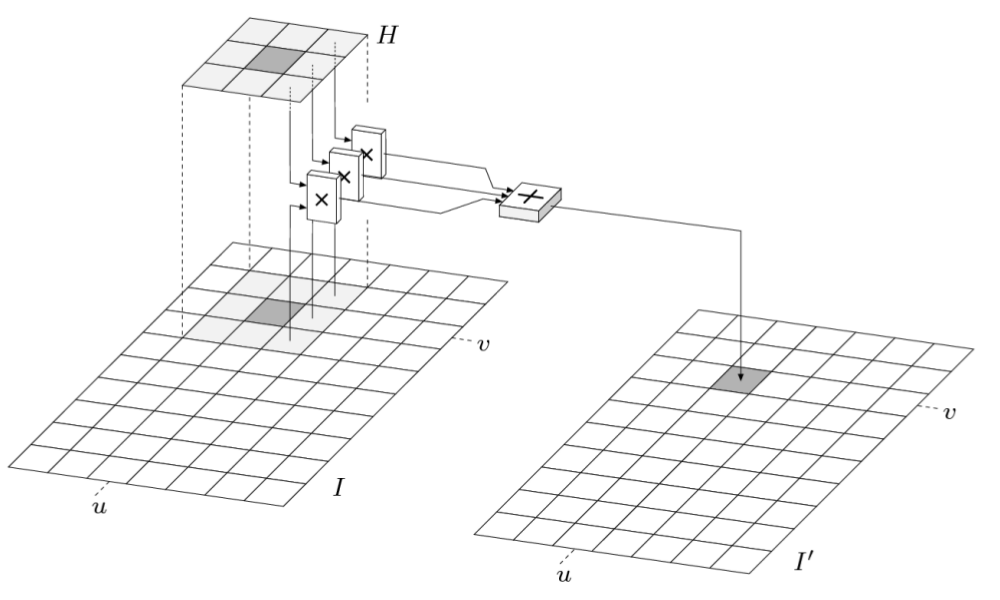
\includegraphics[scale=0.35]{bilder/filter.png}
    	\caption{Darstellung der Filteroperation für ein Bild I und die Filtermatrix H. (Abbildung aus \cite[S. 92]{Burg06})}
    	\label{fig:filter}
\end{figure}

\subsubsection{Gaußfilter}

Der Gaußfilter ist ein Glättungsfilter, bei dem die Werte der Filtermatrix einer diskreten zweidimensionalen Gaußfunktion entsprechnen.

\[
G(x, y, \sigma) = \frac{1}{2\pi\sigma^2} e^{-\frac{(x^2 + y^2)}{2 \sigma^2}}
\]

Je weiter ein Pixel vom betrachteten Punkt entfernt ist, umso geringer ist sein Einfluss auf das Filterergebnis.
Wie stark diese Werte abnehmen lässt sich mit der Standardabweichung $\sigma$ kontrollieren.

\subsubsection{Douglas-Peucker-Algorithmus}
\label{sec:douglas}

Der Douglas-Peucker-Algorithmus ist ein Algorithmus, der einen Streckenzug von Punkten durch weglassen einzelner Punkte approximiert \footnote{\cite{douglasalgorithms}}.
Der Algorithmus startet mit der direkten Verbindung der Endpunkte und fügt rekursiv Zwischenpunkte hinzu, bis eine ausreichend gute Approximation gefunden wurde.

Sei $K = (P_1, P_2, ..., P_n)$ der gegebene Streckenzug mit n Punkten. Zudem wird eine Toleranz $\epsilon$ gewählt.

K wird durch die Strecke $\overline{P_1P_n}$ approximiert. Nun wird geprüft, ob diese Approximation ausreichend ist.
Hierfür werden die inneren Punkte zwischen $P_1$ und $P_n$ betrachtet.

Es wird der innere Punkt $P_m$ mit dem größten Abstand $d_{max}$ zur Strecke $\overline{P_1P_n}$ gesucht.
Die Approximation ist ausreichend, wenn es keine inneren Punkte gibt oder $d_{max} \leq \epsilon$ ist. Wird die Approximation als ausreichend befunden, werden alle inneren Punkte verworfen. Ist die Approximation nicht ausreichen, wird der Streckenzug $K$ in zwei Teilfolgen $K_1 = (P_1, ..., P_m)$ und $K_2 = (P_m, ... , P_n)$ aufgeteilt. Diese beiden Teilfolgen werden nun mit dem gleichen Algorithmus approximiert.

Das Endergebnis besteht aus allen Punkten, die nicht verworfen wurden. Keiner der verworfenen Punkte hat zu dem so enstehenden Streckenzug einen größeren Abstand als $\epsilon$.


\subsubsection{Haar Merkmal}
\label{sec:haar}

Ein Haar Merkmal (Haar-like features) beschreibt den Helligkeitsunterschied von zwei aneinanderliegenden rechteckigen Regionen in einem Bild \footnote{\cite{Viola01rapidobject}}.
Für beide Regionen wird die Summe der Intensität aller Pixel berechnet. Diese beiden Summen werden von einander substrahiert. Der so enstehende Wert für den Helligkeitsunterschied bildet das Haar Merkmal.

Die Wahl der Regionen bestimmt, welche Bildeigenschaften das Merkmal darstellt. Die in Abbildung \ref{fig:haar} dargestellten Regionen sind geeignet, um horizontale bzw. vertikale Kanten zu erkennen.


\begin{figure}[h]
    \centering
		
\includegraphics[scale=0.25]{bilder/haar.png}
    	\caption{Beispiel für zwei Haar Merkmale. Der jeweils schwarze und weiße Bereich markiert die Regionen. }
    	\label{fig:haar}
\end{figure}


\subsubsection{Skalenraum}

Ein Objekt, das von einem Menschen beobachtet wird, weist optisch verschiedene Strukturen auf, abhängig von der Distanz zu diesem Objekt. Wird ein Objekt aus großer Entfernung betrachtet, gehen kleinere Strukturen verloren und nur große Strukturen bleiben bestehen.
So lassen sich z.B. aus der Nähe die Blätter eines Baumes betrachten. Aus einer größeren Entfernung hingegen sind die Blätter nicht mehr zu erkennen und nur die grundlegende Form des Baumes.
Der Begriff der Skalierung beschreibt, wie groß dieser Effekt ist. Je höher die Skalierung, um so weniger Details sind erkennerbar.

Der Skalenraum ist ein Konzept der Bildverarbeitung, das ein Bild in verschiedenen Skalierungen darstellen kann \footnote{\cite{Lindeberg94scale-spacetheory:}}. Hierbei kann die Skalierung durch einen kontinuierlichen Skalenparameter $\sigma$ kontrolliert werden.

Um die Skalierung eines Bildes zu erhöhen, wird das Bild geglättet. Durch diese Glättung werden kleine Strukturen unterdrückt (siehe Abbildung \ref{fig:scaleSpace}). Die Glättung wird mit einem Gaußfilter erzeugt \footnote{\cite{Lindeberg94scale-spacetheory:}}. Der Skalenparameter entspricht hierbei der Standardabweichung des Gaußfilters.

Die Skalenraumfunktion eines Bildes wird als $L(x, y, \sigma)$ definiert. Hierbei bestimmt das $\sigma$ die Skalierung. Es gilt mit $*$ als Faltungsoperation für das Bild $I(x, y)$:

\[
L(x, y, \sigma) = G(x, y, \sigma) * I(x, y)
\] 


Wobei $G(x, y, \sigma)$ die 2-Dimensionale Gauß Funktion ist.

\[
G(x, y, \sigma) =  \frac{1}{2 \pi \sigma^{2}} e^{-\frac{(x^2+y^2)}{2\sigma^2}}
\]

Der Skalenraum lässt sich in sogenannte Oktaven einteilen. Eine Oktave im Skalenraum ist jeweils eine Verdoppelung bzw. Halbierung der Skalierung.

\begin{figure}[h]
    \centering
		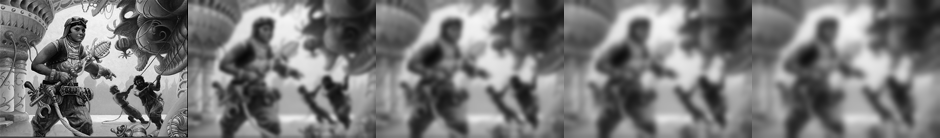
\includegraphics[scale=0.5]{bilder/scaleSpace.png}
    	\caption{Veränderung eines Bildes im Skalenraum. Die Werte für $\sigma$ von links nach rechts: 0, 1.7, 3.4, 5.1, 6.8 und 8.5.}
    	\label{fig:scaleSpace}
\end{figure}


\subsection{Bildmerkmale}

Bildmerkmale stellen eine Möglichkeit dar, bestimmte Punkte oder auch Objekte in einem Bild auf einem anderen Bild wiederzufinden.
Ein einzelnes Merkmal ist eine vektorielle Darstellung eines kleinen Bildbereiches.

Um Merkmale für ein gegebenes Bild zu finden werden zwei Schritte vollzogen.

\begin{itemize}
\item Merkmalsdetektion, findet Punkte im Bild, die sich gut für Merkmale eignen. Diese Punkte werden im Weiteren auch als Keypoints bezeichnet.
\item Merkmalsbeschreibung, wandelt Punkte in eine vektorielle Darstellung um. Im Weiteren auch Deskriptor genannt.
\end{itemize}

Es gibt eine große Anzahl an Methoden, um diese beiden Schritte durchzuführen (siehe Tabelle \ref{table:featureMethods}).
In dieser Arbeit werden die drei Methoden ''Scale-Invariant Feature Transform'' (SIFT), ''Speeded Up Robust Features'' (SURF) und ''Oriented FAST and Rotated BRIEF'' (ORB) betrachtet. 

\begin{table}
\centering
	\begin{tabular}{  l c c   }
	  Methode & Merkmalsdetektion & Merkmalsbeschreibung \\
	  \midrule
	  Harris Corner Detection & X & - \\
	  Features from Accelerated Segment Test & X & - \\
	  Binary Robust Independent Elementary Features & - & X \\
	  Scale-Invariant Feature Transform & X & X \\
	  Speeded-Up Robust Features & X & X \\
	  Oriented FAST and Rotated BRIEF & X & X \\
	  
	\end{tabular}
\caption{Übersicht häufig verwendeter Merkmalsdetektoren und Merkmalsbeschreibern.}
\label{table:featureMethods}
\end{table}

\subsubsection{Merkmalsdetektion}
\label{sec:featureDetection}
Der erste Schritt ist das Finden von Bildausschnitten, die Eigenschaften haben, die möglichst einzigartig sind und sich auch in anderen Bildern wiedererkennen lassen. Diese Merkmale sollen so gewählt werden, dass sie auch nach Rotationen oder Veränderung der Bildgröße bestehen bleiben. Flächen ohne große Veränderungen oder Kanten lassen sich schlecht in Bildern wiederfinden.
Dies lässt sich einfach mit einem Stück blauen Himmel in einem Bild vorstellen. Der Bildausschnitt des Himmels hat keine besonderen Eigenschaften, die ihn einfach von anderen Himmelstücken in Bildern unterscheiden.
Eine Kante hingegen lässt sich deutlich besser wiederfinden. Jedoch ist es bei einem Ausschnitt einer Kante schwer festzustellen, wo sich dieser Ausschnitt entlang der gesamten Kante befindet.
Ecken hingegen sind eindeutiger in einem Bild lokalisierbar.

In Abbildung \ref{fig:featureSample} ist ein Beispiel für die Keypoints, die gefunden werden, zu sehen.

\begin{figure}[h]

    \centering
		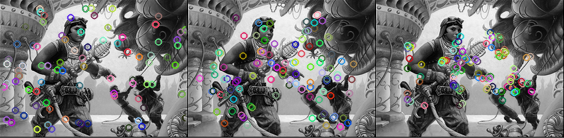
\includegraphics[scale=0.8]{bilder/featureSample.png}
    	\caption{Von links nach rechts die gefundenen Keypoints von SIFT, SURF und ORB. Keypoints sind jeweils mit einem farbigen Kreis markiert. Die Farben haben keine Aussage über den Keypoint und dienen nur der besseren Unterscheidung nahe liegender Punkte. Die Anzahl der gezeigeten Keypoints ist für eine bessere Übersicht jeweils auf 100 beschränkt}
\label{fig:featureSample}
\end{figure}

\subsubsection{Merkmalsdeskription}

Von den Bildausschnitten, die von der Merkmalserkennung als interessant befunden wurden, soll nun in diesem Schritt ein Merkmalsvektor erstellt werden.
Dieser Vektor soll den Ausschnitt so beschrieben, dass für den gleichen Ausschnitt aus einem anderen Bild der Deskriptorvektor sehr ähnlich ist.


\subsubsection{Merkmalsabgleich}

Nachdem die Merkmalsvektoren für interessante Bildausschnitte erstellt wurden, kann nun versucht werden, Merkmale aus einem Bild in einem anderen wiederzufinden.
Da die Vektoren so konstruiert sind, dass ähnliche Bereiche zu ähnlichen Vektoren führen, kann ein Merkmal eines Bildes in einem anderen wiedergefunden werden, indem man den Vektor mit der geringsten Distanz findet.


In Abbildung \ref{fig:matchingSample} ist ein Beispiel für den Merkmalsabgleich zu sehen. Die Merkmale des gedrehten Bildes werden in denen des nicht gedrehten wiedergefunden werden.

\begin{figure}[h]

    \centering
		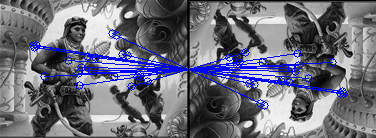
\includegraphics[scale=0.8]{bilder/matchingSample.png}
    	\caption{Die zusammengehörigen Keypoints sind jeweils mit einer Linie verbunden. Die Zahl der gezeigten Matches ist zur besseren Übersicht auf 20 beschränkt.}    	\label{fig:matchingSample}
\end{figure}


\subsubsection{Features from Accelerated Segment Test}
\label{sec:fast}

Das in Edward Rostens und Tom Drummonds Paper ''Machine learning for high-speed corner detection'' \footnote{\cite{Rosten:2006:MLH:2094437.2094478}}  vorgestellte Verfahren ''Features from Accelerated Segment Test'' (FAST) ist ein Merkmalsdetektor.

Damit ein Punkt $p$ mit Intensität $I_p$ als Keypoint erkannt wird, betrachtet FAST einen Kreis um den Punkt. Es wird geprüft, ob es in diesem Kreis eine Menge mit $n$ zusammenhängenden Pixeln gibt, die eine der folgenden Bedingungen erfüllt:

\begin{itemize}
\item Die Intensität jedes Pixels in der Menge ist kleiner als $I_p - t$, wobei t eine konstante Schwelle ist
\item Die Intensität jedes Pixels in der Menge ist größer als $I_p + t$, wobei t eine konstante Schwelle ist
\end{itemize}

Ist eine dieser Bedingunen erfüllt, wird der Punkt als Keypoint erkannt.

\subsection{Weitere Methoden}

\subsubsection{k-nächste-Nachbarn}
\label{sub:knn}

Der k-nächste-Nachbarn (k-Nearest-Neighbors) Algorithmus ist eine Klassifikationsmethode, mit der neue Datenpunkte anhand schon bekannter Daten klassifiziert werden können \footnote{\cite{doi:10.1080/00031305.1992.10475879}}.

Sei $x \in \mathbb{R}^n$ der neue Datenpunkt, der einer von $m \in \mathbb{R}$ verschiedenen Klassen zugeordnet werden soll. Zudem sei $D \subseteq \mathbb{R}^n$ die Menge an Punkten, deren wahre Klasse bekannt ist.

\begin{figure}[h]
    \centering
		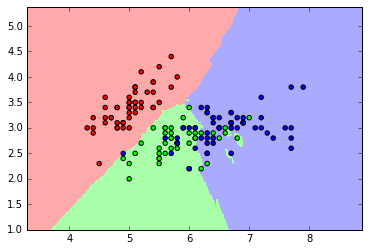
\includegraphics[scale=0.45]{bilder/knn.png}
    	\caption{k-nächste-Nachbarn Klassifikation für drei Klassen (Rot, Blau, Grün). Die Datenpunkte jeder Klasse sind farblich eingezeichnet. Die farbigen Bereiche zeigen an, wie ein neuer Datenpunkt klassifiziert wird, wenn er in diesen liegt.}
    	\label{fig:knn}
\end{figure}

Nun wird ein $k$ gewählt und die $k$ nächsten Nachbarn von x in $D$ gesucht. Nun wird $x$ die Klasse zugewiesen, die durch eine einfache Mehrheitswahl der k nächsten Nachbarn bestimmt wird.
Eine Visualisierung dieser Klassifikation ist in Abbildung \ref{fig:knn} dargestellt.

\subsubsection{Hamming Distanz}
\label{sub:hammingDistanz}

Die Hamming Distanz ist eine Methode, mit der die Ähnlichkeit von zwei gleichlangen Zeichenketten gemessen werden kann \footnote{\cite{hamming}}.
Sie ist definiert als die Anzahl der unterschiedlichen Stellen in den beiden Zeichenketten. 
Die Hamming Distanz kann auch genutzt werden, um die Binärdarstellung zweier Zahlen zu vergleichen. So ist z.B. die Hamming Distanz von $1001$ und $0000$:
\[
H(1001, 0000) = 2
\]


\subsection{Scale-Invariant Feature Transform (SIFT)}
Das folgende Kapitel basiert auf David G. Lowes Paper ''Distinctive Image Features
from Scale-Invariant Keypoints'' \footnote{\cite{Lowe2004}}

In seinem Paper ''Distinctive Image Features from Scale-Invariant Keypoints'' von 2004 stellte David G. Lowe eine Methode zur Merkmalsfindung und Merkmalsbeschreibung vor.

Das Verfahren wurde mit dem Ziel entworfen, dass Merkmale unabhängig von Rotation und Skalierung gefunden werden. So sollen Objekte in Bildern wiedergefunden werden können, wenn sie gedreht oder näher bzw. weiter weg sind.

Die SIFT Merkmale werden in 4 Schritten berechnet.

\begin{enumerate}

\item Extrema im Skalenraum finden, die potentielle Keypoints sein können
\item Prüfen, ob die zuvor gefundenen Punkte geeignete Keypoints sind
\item Zuweisen einer Orientierung für den Bildausschnitt
\item Erstellen des Deskriptors

\end{enumerate}

\subsubsection{Merkmalserkennung}

Da SIFT versucht Merkmale zu finden, die für verschiedene Skalierungen des Bildes konstant sind, müssen Punkte gefunden werden, die invariant zur Skalierung des Bildes sind.
Für die Erkennung von Merkmalen soll sich also nicht auf Details, die in höheren Skalierungen verloren gehen verlassen, sondern Punkte gefunden werden, die im Skalenraum Extrema sind.

Es wurde von Lowe gezeigt \footnote{\cite{Lowe:1999:ORL:850924.851523}}, dass Merkmale im Skalenraum durch Extrema der Differenz der Gauß Funktionen gefunden werden können.
Sei $I(x, y)$ das Bild, $G(x, y, \sigma)$ die zwei Dimensionale Gaußfunktion  und $L(x, y, \sigma)$ die Skalenraumfunktion.
Die Differenz der Gaußfunktionen $D(x, y, \sigma)$ für zwei Skalierungen, die um einen Faktor $k$ im Skalenraum entfernt sind, ist definiert als:

\[
D(x, y, \sigma) = G(x, y, k\sigma) - G(x, y, \sigma)) * I(x, y)\\ = L(x, y, k\sigma) - L(x, y, \sigma)
\]

Die Differenz der Gaußfunktionen zeigt, welche Strukturen in dem Übergang von einer Skalierung in die andere verloren gehen. In Abbildung \ref{fig:dogSample} ist dies für das Bild aus Abbildung \ref{fig:scaleSpace} dargestellt.

\begin{figure}[h]
    \centering
		
\includegraphics[scale=0.55]{bilder/firstDiv.png}
    	\caption{Differenz der Gaußfunktionen aus Abbildung \ref{fig:scaleSpace}. Die weißen Bereiche zeigen die Bereiche an, in denen Details verloren gehen.}

\label{fig:dogSample}
\end{figure}


Um die Differenz der Gaußfunktionen effizient zu berechnen, wird das Eingabebild mehrmals mit der Gaußfunktion gefaltet, um mehrere Skalierungen des Bildes zu erzeugen. Die einzelnen Skalierungen liegen immer um den Faktor $k$ auseinander.  Es werden jeweils von 2 Skalierungen, die im Skalenraum nebeneinander sind, die Differenz gebildet.
Sobald eine Oktave im Skalenraum durchlaufen ist, wird die Auflösung des Ursprungsbildes der Oktave halbiert. Dieses Bild bildet den Anfang der nächsten Oktave.
Dieser Vorgang wird in Abbildung \ref{fig:siftDog} dargestellt.

\begin{figure}[h]
    \centering
		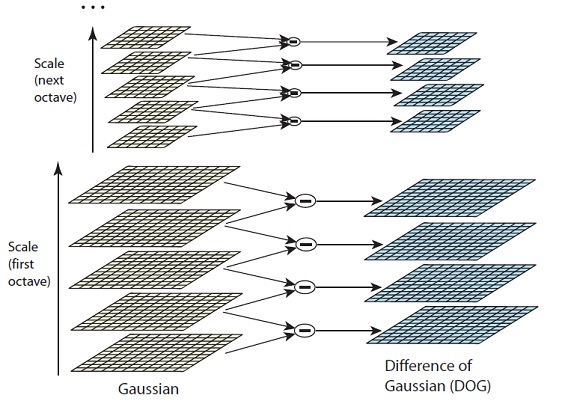
\includegraphics[scale=0.8]{bilder/sift-dog-idea.jpg}
    	\caption{Differenz der Gaußfunktionen für verschiedene Skalierungen und Oktaven (Abbildung aus \cite[S. 6]{Lowe2004}).}
\label{fig:siftDog}
\end{figure}

Um nun lokale Extrema im Scale Space zu finden, werden viele Beispielpunkte aus verschiedenen Skalierungen und Oktaven gewählt. Es werden drei Skalierungen pro Oktave betrachtet. Die Oktaven werden weitergeführt, bis die Bildauflösung zu gering ist.

Für jeden Punkt wird nun überprüft, ob er ein lokales Extremum ist. Dafür wird geprüft, ob der Punkt größer oder kleiner als alle seine Nachbarn in seiner eigenen Skalierung und in den Skalierungen darüber und darunter ist.

\begin{figure}[h]
    \centering
		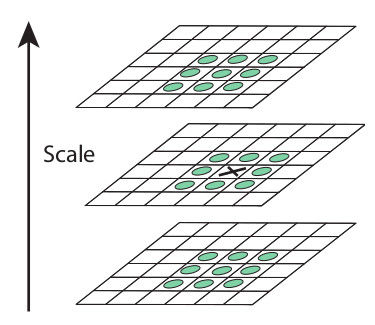
\includegraphics[scale=0.4]{bilder/sift_extrema.png}
    	\caption{Um ein Extremum zu sein, muss der mit X markierte Punkt größer oder kleiner sein als alle Nachbarn in anliegenden Scales (Abbildung aus\cite[S. 7]{Lowe2004}).}
\end{figure}

Viele der so gefunden Punkte sind nicht geeignet um stabile Merkmale zu sein:

Punkte mit zu geringem Kontrast (\ref{sec:kontrast}) sind nicht robust gegenüber Bildrauschen (\ref{sec:rauschen}). Durch den geringen Kontrast kann bereits leichtes Bildrauschen den Bereich stark verfälschen.
Deshalb werden von den potentiellen Merkmalen alle Punkte, deren Umgebung einen zu geringen Kontrast aufweist, entfernt.

Wie in \ref{sec:featureDetection} erwähnt, lassen sich Punkte entlang Kanten nicht gut an der Kante lokalisieren.

Der Gradient an Punkte, die an einer Kante liegen, ist in die Richtung der Kante sehr gering und in die Richtung entgegen der Kante sehr groß. Bei einer Ecke hingegen sind die Gradienten in alle Richtungen groß.
Für den Punkt wird die Richtung mit dem größten Gradienten gesucht und die Richtung rechtwinkling zu dieser. Ist das Verhältnis der Gradienten in die beiden Richtungen groß, so liegt der Punkt an einer Kante.

Um Punkte entlang Kanten zu entfernen, wird die Krümmung an dem jeweiligen Punkt betrachtet. Als Krümmung wird in diesem Zusammenhang die Ableitung der Gradiente verstanden. Die Richtung, in die die Krümmung am stärksten ist, wird als Hauptkrümmung bezeichnet.
Eine Kante hat eine starke Krümmung rechtwinklig zur Kante. Jedoch ist die Krümmung in Richtung der Kante sehr klein. 
Es wird nun das Verhältnis der Hauptkrümmung und der Krümmung rechtwickling zur Hauptkrümmung betrachtet.
Bei einer Ecke sind beide Krümmungen groß, also der Quotient der beiden gering. Bei einer Kante ist nur die Hauptkrümmung groß. Dadurch ist auch der Quotient groß. 
Ist das Verhältnis der beiden Krümmungen zu groß, wird der Punkt nicht mehr weiter betrachtet.


Die übrig gebliebenen Punkte werden nun Orientierungen zugewiesen und verwendet, um Merkmale zu bilden.


Um einem Punkt eine Orientierung zuzuweisen, wird für eine Region um ihn die Richtung $\theta(x, y)$ und Größe $m(x, y)$ der Gradienten berechnet. Das $\sigma$ entspricht der Skalierung, in der der Punkt gefunden wurde.
\[
m(x, y) = \sqrt{(L(x + 1, y, \sigma) - L(x - 1, y, \sigma))^2 + (L(x, y + 1, \sigma) - L(x, y - 1, \sigma))^2}
\]

\[
\theta(x, y)) = \tanh^{-1}((L(x + 1, y, \sigma) - L(x - 1, y, \sigma)) / (L(x, y + 1, \sigma) - L(x, y - 1, \sigma)))
\]

Es wird nun ein Histogramm der Gradientenrichtungen gebildet. Dieses Histogramm hat 36 Klassen, die jeweils 10° abdecken. Bei jedem hinzugefügten Punkt aus der Region wird dieser mit dem Gewicht $m(x, y)$ und einer Gaußgewichtung um den Ursprungspunkt des Ausschnittes gewichtet.
Aus dem Histogramm können nun durch die Spitzen die Orientierung der Region abgelesen werden. Sollte eine weitere Spitze nicht kleiner als 80\% der größten Spitze sein, wird für diese auch ein Merkmal erstellt. So enstehen für Regionen mit mehren Hochpunkten im Richtungshistogramm auch mehrere Merkmale.

\subsubsection{Merkmalsbeschreibung}

Nachdem einem Bildausschnitt eine Skalierung und eine Orientierung zugeordnet wurde, wird in diesem Schritt eine vektorielle Darstellung von diesem Aussschnit erstellt.


Der Deskriptor wird für eine $16 \times 16$ Umgebung um den Punkt gebildet. Hierbei wird für jeden Pixel in der Umgebung die Richtung $\theta(x, y)$ und Stärke $m(x, y)$ des Gradienten berechnet. Die Richtung wird um die zuvor gefundene Rotation gedreht, damit eine Unabhängigkeit von der Rotation gegeben ist.

Die Gradienten werden mit einem Gaußfenster gewichtet und in $4 \times 4$ Regionen eingeteilt (siehe Abbildung \ref{fig:siftDesc}). In diesen Regionen werden die Gradienten einer von 8 Richtungen zugeordnet, der sie am nächsten sind. Damit bildet jede Region einen 8 dimensionalen Merkmalsvektor. Der enstehende Deskriptor für den Bildausschnitt ist somit $4 \times 4 \times 8$.



\begin{figure}[h]
    \centering
		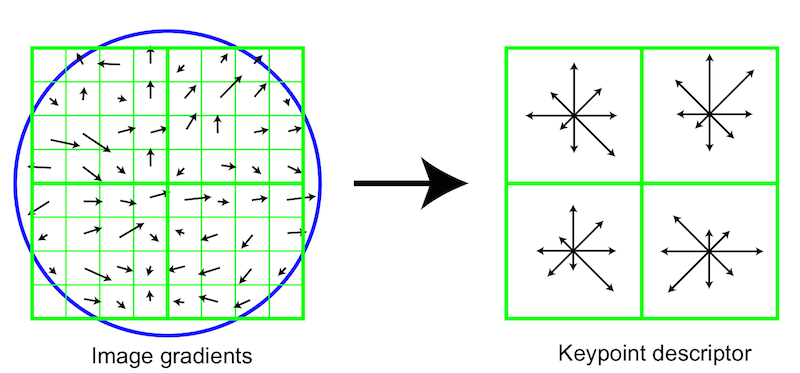
\includegraphics[scale=0.8]{bilder/sift_pic.png}
    	\caption{Umwandlung der Gradienten in den Descriptor für einen $8 \times 8$ Bildausschnitt. SIFT benutzt einen $16 \times 16$ Ausschnitt, aus dem ein $4 \times 4$ Descriptor erstellt wird.  Der blaue Kreis stellt die Gaußgewichtung dar (Abbildung aus\cite[S. 15]{Lowe2004}).}
 \label{fig:siftDesc}
\end{figure}



\subsection{Speeded Up Robust Features (SURF)}
Das Folgende Kapitel basiert auf dem Paper ''SURF: Speeded Up Robust Features'' von Herbert Bay.
\footnote{\cite{Bay:2008:SRF:1370312.1370556}}

Das Verfahren ''Speeded Up Robust Features'' (SURF) wurde von Herbert Bay 2006 vorgestellt. SURF ist ein Verfahren, das sowohl Merkmale findet, als auch Deskriptoren für diese bildet.
SURF versucht durch einige Approximationen schneller als SIFT zu sein ohne große Verluste in der Genauigkeit zu haben.

Für schnelle Berechnung von rechteckigen Filtern werden Integralbilder verwendet. Diese ermöglichen eine sehr schnelle Berechnung von Pixelsummen in einem rechteckigen Bildbereich.
In einem Integralbild ist jeder Pixelwert die Summe aller Pixel in einem Rechteck zwischen dem aktuellen Punkt und dem Bildursprung.

\[
I_i(x, y) = \sum_{i = 0}^{i < x} \sum_{j = 0}^{j < y} I(i, j)
\]

Nun kann die Summe der Pixelwerte eines Recktecks
 $R = \{ (x_1, y_1), (x_2, y_2), (x_3, y_3), (x_4, y_4)  \}$ mit nur vier Bildzugriffen berechnet werden.
\[
S(R) = I_i(x_1, y_1) + I_i(x_4, y_4) - I_i(x_2, y_2) - I_i(x_3, y_3)
\]



\subsubsection{Merkmalserkennung}

SURF nutzt die Determinante der Hesse-Matrix um Keypoints zu finden. Die Hesse-Matrix ist die zweite Ableitung einer mehrdimensionalen Funktion. Sie kann somit als ein Maß der Krümmung verstanden werden.
Es wird, ähnlich zu SIFT, in verschiedenen Skalierungen nach Maxima von $det(\mathcal{H}(x, y, \sigma))$ gesucht. Dabei ist die Hesse Matrix $\mathcal{H}(x, y, \sigma)$ für das Bild $I(x, y)$ und die Skalierung $\sigma$ definiert als:

\[
\mathcal{H}(x, y, \sigma) = 
\begin{bmatrix}
L_{xx}(x, \sigma) & L_{xy}(x, \sigma) \\
L_{xy}(x, \sigma) & L_{yy}(x, \sigma)
\end{bmatrix}
\]

Wobei $L_{xx}(x, y, \sigma)$ die Faltung von der zweifachen nach x abgeleiteten Gaußfunktion mit dem Bildpunkt ist. Das gleiche gilt für $L_{xy}(x, y, \sigma)$ und $L_{yy}(x, y, \sigma)$ in die entsprechenden Richtungen.

Um die Determinante schnell berechnen zu können, werden die partiellen Gaußableitungen mit rechteckigen Filtern approximiert. Diese seien im Folgenden $D_{xx}$, $D_{xy}$ und $D_{xy}$. Für die kleinste Skalierung $\sigma = 1.2$ wird ein $9x9$ Filter verwendet (siehe Abbildung \ref{fig:surfBox}).

SURF approximiert die Determinante mit 

\[
det(\mathcal{H}_{approx}(x, y, \sigma)) = D_{xx}D_{yy} - (0.9 D_{xy})^2
\]

In SIFT werden Gaußfilter mehrfach auf ein Bild angewandt, um höhere Skalierungen zu erhalten.
Der gleiche Effekt kann durch eine Erhöhung der Größe des Gaußfilters erreicht werden. Durch Integralbilder lässt sich die Filtergröße erhöhen, ohne mehr Berechnungen zu machen.
So nutzt SURF für die erste Oktave Filter der Größe $9x9, 15x15, 21x21, 27x27$. Der Abstand zwischen den Filtergrößen wird jede Oktave verdoppelt.


\begin{figure}[h]
    \centering
		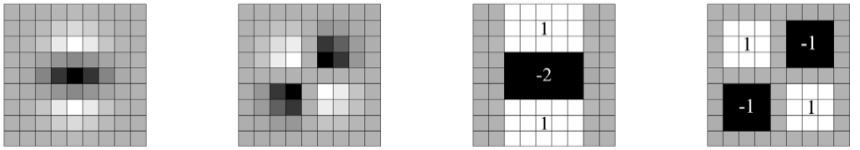
\includegraphics[scale=0.4]{bilder/surfBoxFilter.png}
    	\caption{Die Gaußfilter für die y und xy Richtung sowie deren Approximationen (Abbildung aus \cite{Bay:2008:SRF:1370312.1370556}).}
\label{fig:surfBox}
\end{figure} 


Um nun Keypoints in den verschiedenen Skalierungen zu finden, wird wie in SIFT geprüft, ob $det(\mathcal{H}(x, y, \sigma))$ an einem  Punkt in einer $3x3x3$ Nachbarschaft das Maximum ist.



\subsubsection{Merkmalsbeschreibung}

Der erste Schritt zur Erstellung des Deskriptors ist, dem Punkt eine Orientierung zuzuordnen. Sei $s$ im folgenden die Skalierung, in dem der Keypoint gefunden wurde.

Um dem Punkt eine Orientierung zuzuweisen, werden Haar Merkmale (siehe \ref{sec:haar}) verwendet. 
Es werden jeweils die Haar Merkmale in x und y Richtung bestimmt. Hierfür werden die Regionen in Abbildung \ref{fig:haar} mit einer Seitenlänge von $4s$ verwendet. Durch die Verwendung von Integralbildern sind diese Berechnungen sehr effizient.


Mit der gefunden Orientierung wird ein $20s$ großes Quadrat um den Punkt gelegt, welches um die Orientierung gedreht wird.
Dieses Quadrat wird in $4 \times 4$ Regionen unterteilt. In diesen Regionen wird ein 4-dimensionaler Merkmalsvektor bestimmt. Dieser Vektor besteht aus den Summen der horizontalen und vertikalen Haar Merkmale $dx$ und $dy$ in der Region(siehe Abbildung \ref{fig:surfFeature}). 
Die Größe der Regionen wird als $2s$ gewählt. Der Vektor ist definiert als: 

\begin{figure}[h]
    \centering
		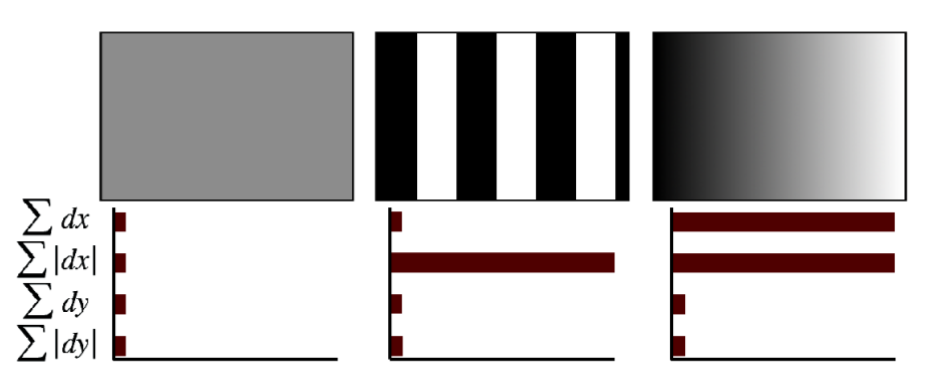
\includegraphics[scale=0.4]{bilder/surfFeature.png}
    	\caption{Die Größe der jeweiligen Merkmale für die gezeigten Bildausschnitte. Die einzelnen Komponenten des Vektors beschreiben die Strukturen der Intensität (Abbildung aus \cite{Bay:2008:SRF:1370312.1370556}).}
\label{fig:surfFeature}
\end{figure} 


\[
v = (\sum dx, \sum  |dx|, \sum dy, \sum |dy|)
\]

Aus den $4 \times 4$ Vektoren der einzelnen Regionen wird der Gesamtdeskriptor für das Merkmal gebildet.
Dadurch ensteht für jedes Merkmal ein 64-dimensionaler Vektor, der dieses Merkmal beschreibt.

\subsection{Oriented FAST and Rotated BRIEF (ORB)}
Das folgende Kapitel basiert auf dem von Ethan Ruble veröffentlichtem Paper ''ORB: an efficient alternative to SIFT or SURF'' \footnote{\cite{Rublee:2011:OEA:2355573.2356268,}}.

ORB wurde 2011 von Ethan Ruble als eine alternative zu SIFT und SURF vorgestellt, die deutlich schneller sein und dabei jedoch eine vergleichbar gute Perfomance haben sollte.
ORB kombiniert mehrere bestehende Verfahren und erweitert diese, um mit Rotation umgehen zu können. So wird FAST und ein Harris-Corner Detector \footnote{\cite{Harris88alvey}} verwendet, um Keypoints zu finden. Zudem werden die ''Binary Robust Independent
Elementary Features'' (BRIEF) \footnote{\cite{Calonder:2010:BBR:1888089.1888148,}} für die Merkmalsbeschreibung verwendent und so erweitert, dass sie mit der Rotation von Bildausschnitten umgehen können.

\subsubsection{Merkmalserkennung}

Um eine erste Auswahl an möglichen Keypoints zu erhalten wird FAST (siehe \ref{sec:fast}) verwendet.


FAST findet jedoch auch viele Punkte, die an einer Kante liegen und keine Ecke sind. Um diese herauszufiltern, wird der Harris-Corner Detector verwendet. Dieser gibt für einen Punkt ein Maß an, wie sehr dieser Punkt eine Ecke ist \footnote{\cite{Harris88alvey}}.


Für alle von FAST gefundenen Punkte wird der Harris Wert berechnet.
Um eine gewisse Anzahl $N$ an Punkten zu finden, wird  eine Schwelle $t$ zuerst so klein gewählt, dass mehr als $N$ Punkte über dieser liegen. Diese Punkte werden dann nach ihrem Harris Wert geordnet und die $N$ größten ausgewählt.
Damit die Merkmale Skalierungsinvariant sind, wird dies für mehrer Skalierungen des Bildes durchgeführt.

Da die von FAST gefundenen Punkte keine Orientierung haben, wird jedem gefundenen Merkmal noch eine Orientierung zugewiesen.
Dafür wird der Intensitätsschwerpunkt genutzt. Dieser liegt bei einer Ecke versetzt vom Mittelpunkt des betrachteten Bildausschnitts.
Um den Intensitätsschwerpunkt zu finden, werden die Momente des Ausschnittes betrachtet.
Momente in der Bildverarbeitung sind gewichtetete Intensitäten der Pixel eines Bildes bzw. eines Bildausschnittes.
Der Moment des $p$ und $q$ Grades, mit $p, q \in \mathbb{R}$ ist definiert als:

\[
m_{pq} = \sum_{x, y} x^p y^q I(x, y)
\]

Aus den Momenten $m_{00}, m_{01}$ und $m_{10}$ lässt sich der Schwerpunkt bestimmen.

\[
C =  \bigg(\frac{m_{10}}{m_{00}} , \frac{m_{01}}{m_{00}}\bigg)
\]

Die Orientierung des Keypoints wird definiert als der Vektor vom Zentrum bis zum Intensitätsschwerpunkt (siehe Abbildung \ref{fig:centroid}).

\begin{figure}[h]

    \centering
		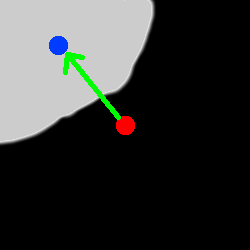
\includegraphics[scale=0.65]{bilder/centroid.png}
    	\caption{Der rote Punkt ist das Zentrum des Bildausschnitts und der blaue Punkt markiert den Intensitätsschwerpunkt. Der grüne Vektor zwischen den beiden bestimmt die Orientierung des Bildausschnitts.}
\label{fig:centroid}
\end{figure}


\[
\theta = \atantwo (m_{01}, m_{10})
\]

Diese Orientierung wird in $2\pi / 30$ große Abschnitte unterteilt.

\subsubsection{Merkmalsbeschreibung}

Um einen Deskriptor für ein gefundenes Merkmal zu bilden, wird ein $31 \times 31$ Bildausschnitt $p$ um den Keypoint betrachtet.
ORB benutzt eine um Rotation erweiterte Variante von BRIEF.
BRIEF erstellt einen binären Vektor aus einfachen Intensitätsvergleichen von zwei Bildpunkten. Hierfür wird der Bildausschnitt $p$ zuerst mit einem Gaußfilter geglättet.

Der binäre Test $\tau$ für den Bildausschnit $p$, wobei $p(x)$ die Intenstität an Bildpunkt x ist, ist definiert als:

\[
\tau(p; x, y) = 
\begin{cases}
1, & p(x) < p(y) \\
0, & p(x) \geq p(y)
\end{cases}
\]

Die Bitfolge der Testergebnisse ergibt sich aus:

\[
f_n(p) = \sum_{1 \leq i \leq n} 2^{i-1} \tau (p; x_i, y_i)
\]



Definiere die $2 \times n$ Matrix $S$ für alle n Vergleichspunkte $(x_i, y_i)$:

\[
S = \begin{pmatrix}
x_1 & \hdots & x_n \\
y_1 & \hdots & y_n 
\end{pmatrix}
\]

Für den Winkel $\theta$ des Bildausschnitts wird die Rotationsmatrix $R_\theta$ definiert, welche die Punkte in $S$ um $\theta$ dreht.

\[
S_\theta = R_\theta S
\]


\[
g_n(p, \theta) = f_n(p)|(x_i, y_i) \in S_\theta
\]


In der $31 \times 31$ Umgebung um den Keypoint gibt es eine hohe Anzahl an Bildpunkten, die miteinander verglichen werden könnten. Von all diesen Paaren $(x, y)$ sollen 256 ausgewählt werden.
Damit der Deskriptor möglichst diskriminierend ist, sollen Paare gewählt werden, die für eine große Menge an Bildausschnitten, auf denen sie ausgeführt werden, folgenden Eigenschaften haben:
\begin{itemize}

\item  Der Mittelwert des Testergebnisses liegt möglichst nah an $0.5$, also liefert der Test für verschiedene Bilder oft verschiedene Ergebnisse

\item Die Korrelation zwischen den gewählten Tests sollte möglichst gering sein, sodass jeder Test neue Informationen hinzubringt

\end{itemize}

Um die Testpaare zu lernen nutzt ORB ein Trainingsset von ca. 300000 Merkmalen aus dem PASCAL 2006 Bildersatz. Eine Auswahl der gelernet Testpaare ist in Abbildung \ref{fig:orbPairs} dargestellt.

\begin{figure}[h]

    \centering
		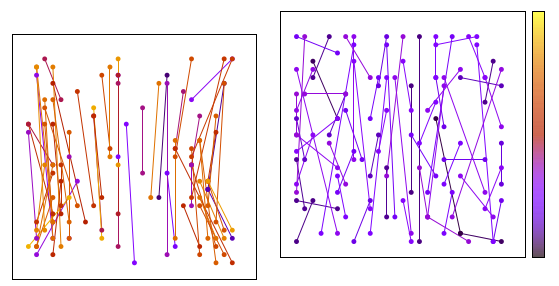
\includegraphics[scale=0.5]{bilder/orbPairs.png}
    	\caption{Darstellung einer Auswahl an Testpaaren. Die linke Seite zeigt Testpaare, die eine hohe Varianz besitzen. Die rechte Seite zeigt die Tests, nachdem der Trainingsschritt abgeschlossen wurde. Die Farben zeigen die maximale Korrelation eines Tests an. Schwarz und Lila stellen die geringste Korrelation dar. }
\label{fig:orbPairs}
\end{figure}

Es werden zuerst alle möglichen Testpaare für alle Keypoints berechnet und nach dem Abstand ihres Mittelwertes zu $0.5$ sortiert. 
Zunächst wird der Test, dessen Mittelwert am nächsten an $0.5$ dran ist, in die Ergebnismenge hinzugefügt.


Nun wird die sortierte Liste an Testpaaren durchgelaufen und ein Test zur Ergebnissmenge hinzugefügt wenn, seine Korrelation unter einem Schwellwert liegt. Ist das der Fall, wird der Test aus der sortierten Liste entfernt. Dies wird solange durchgeführt bis 256 Tests in der Ergebnismenge sind. 
Wird die Liste komplett durchlaufen und die Ergebnismenge ist kleiner als 256, wird der Schwellwert verringert und die Liste noch einmal neu durchlaufen.

Die so gefundenen 256 Testpaare bilden nun den ORB Deskriptor.

\section{Anwendung}\raggedbottom 

Es sollen Karten in Videobildern erkannt werden. Dies soll über die Merkmale der Karten ermöglicht werden. Hierbei werden die Merkmale verwendet, die die Verfahren SIFT, SURF und ORB finden. Es soll verglichen werden, wie groß die Erkennungsrate für die Merkmale der einzelnen Verfahren ist.

Es wird ein Trainingsdatensatz erstellt, aus dem die Merkmale der einzelnen Karten berechnet werden.
Zudem wird ein Klassifikator vorgestellt, der mit Merkmalsabgleichen zwischen dem Bild einer unbekannten Karte und dem Trainingsdatensatz die unbekannte Karte klassifizieren kann.
Ein händisch erstellter Testdatensatz wird verwendet, um die Erkennungsrate des Klassifikators in Verbindung mit den von SIFT, SURF und ORB gefunden Merkmalen zu testen. Hierbei soll das beste Verfahren in Bezug auf Erkennungsrate und Geschwindigkeit gefunden werden.


\subsection{Aufbau einer Karte}

\begin{figure}[h]
    \centering
		
\includegraphics[scale=0.5]{bilder/sampleCard.png}
    	\caption{Beispielkarte ''Aviary Mechanic''}
    	\label{fig:sampleCard}
\end{figure}

Damit Karten identifiziert werden können, ist es wichtig den Aufbau einer Karte zu verstehen. So können Elemente gewählt werden, die geeignet sind, um Karten zu vergleichen.

Im Folgenden wird der Aufbau anhand der Karte in Abbildung \ref{fig:sampleCard} erklärt, ohne zu sehr auf die Regeln des Spieles einzugehen.

In der obersten Zeile der Karte findet sich der Kartenname  ''Aviary Mechanic'' und rechtsbünding die Kosten der Karte im Spiel. Der Name ist hierbei für jede Karte einzigartig, jedoch gibt es sehr viele andere Karten mit denselben Kosten.
Unter der Kopfzeile befindet sich das Kartenbild. Es ist einzigartig für eine Karte und wird später genutzt, um Karten in Videos zu erkennen.
Die Zeile unter dem Kartenbild beinhaltet den Typ 'Creature' und weitere Subtypen 'Dwarf Artificer' einer Karte und auf der rechten Seite ein Editionssymbol. Da es viele Karten mit dem gleichen Typ und aus der gleichen Edition gibt, sind diese auch nicht geeignet, um die Karte zu erkennen.
Unter dieser Zeile befindet sich ein großes Textfeld, welches den Regeltext der Karte beinhaltet.
Unten rechts befindet sich die ''Power'' und ''Toughness'' einer Kreatur. Da es viele Karten mit den gleichen Werten gibt, lässt sich diese Zahl auch nicht zum Erkennen nutzen.

Karten gehören im Spiel immer zu einer oder mehreren "Farben" (Weiß, Blau, Schwarz, Rot, Grün oder farblos). Der Kartenhintergrund entspricht jeweils dieser Farbe oder ist golden, wenn eine Karte zu mehren Farben gehört.
Jede Karte besitzt einen schwarzen Rand. Dieser wird später dafür verwendet Karten aus einem Spielbild zu lokaliseren. 

\subsubsection{Verwendbare Eigenschaften}

Von allen Elementen auf einer Karte sind nur Name und Bild in der Lage die Karte eindeutig zu indentifizieren. Der Name ist auf dem Videomaterial aufgrund der geringen Auflösung einer einzelnen Karten nicht lesbar.
Somit bleibt das Bild als einzige Möglichkeit, eine Karte aus einem Videobild eindeutig zu klassifizieren.


\subsection{Trainingsdatensatz}

Um Karten durch Merkmalsabgleiche zu erkennen, wird zuerst ein Datensatz an Karten benötigt, deren Klasse bekannt ist. Die Klasse ist in diesem Zusammenhang der Name der Karte. Über diesen Datensatz werden die Merkmale der einzelnen Karten berechnet, welche später mit den Merkmalen aus dem Testdatensatz verglichen werden.

\subsubsection{Aufbau}

Der Trainingsdatensatz besteht aus allen Karten der Edition ''Kaladesh'' und umfasst somit 264 Bilder. Jede Karte stellt eine eigene Klasse dar. Für jede Karte ist ein gelabeltes Bild vorhanden. Hierbei ist das Label der Name der Karte. Die Bilder haben alle eine Auflösung von $223 \times 311$ Pixeln.


\subsubsection{Erstellung}

Die Kartenbilder stammen von der offiziellen Seite von Wizards of the Coast. Jede Karte besitzt eine ID, mit welcher sich das Bild unter http://gatherer.wizards.com/Handlers/Image.ashx?multiverseid=ID\&type=card finden lässt.

Die Karten werden automatisch über ein Python Skript heruntergeladen. Dieses lädt zuerst für alle angegeben Editionen eine JSON Datei runter, die alle Informationen zu den Karten enthält. Aus dieser Datei werden die Karten IDs herausgelesen und über den oben genannten Link heruntergeladen und benannt.

\subsubsection{Vorverarbeitung}

Bevor mit SIFT, SURF und ORB die Features einer Karte aus dem Trainigsdatensatz gebildet werden, wird eine Vorverarbeitung durchgeführt, um später im Matching mit den Testdaten gute Ergebnisse zu erhalten.

Zuerst wird das Bild der Karte zugeschnitten, sodass nur noch der Bildbereich der Karte vorhanden ist. Dieser zugeschnittene Bereich ist $138 \times 188$ Pixel groß. Alle weiteren Operationen werden auf diesem Ausschnitt ausgeführt.
Das Bild wird auf eine Größe von $128 \times 128$ skaliert und in ein Graubild umgewandelt, da die drei Merkmalsverfahren mit Graubildern arbeiten.
In einem letzen Schritt wird das Bild noch mit einem $5 \times 5$ Gauß-Filter geglättet.

\subsection{Testdatensatz}

Der Testdatensatz besteht aus Bildern von Karten, die händisch aus Videos ausgeschnitten wurden. Die Karten stammen, so wie der Trainingsdatensatz, alle aus der Edition ''Kaladesh''. Er wird genutzt, um die Erkennungsrate der verschiedenen Verfahren beim Merkmalsabgleich zu bestimmen.

\subsubsection{Aufbau}
\label{sub:aufbau}

Der Testdatensatz besteht aus einem Grunddatensatz und drei aus diesem generierten Datensätzen.
Der Grunddatensatz besteht aus 300 benannten Bildern. Diese wurden per Hand aus Videobildern herausgeschnitten und klassifiziert. Die Bilder sind mit einer Auflösung von $85 \times 120$ Pixeln deutlich kleiner, als die Bilder des Trainingsdatensatzes.
Um die Größe des Datensatzes zu erhöhen und die Robustheit der Verfahren gegen häufig auftretende Bildveränderungen zu testen, wird der Datensatz künstlich erweitert.
Hierfür werden zwei Veränderungen betrachtet, die bei dem Videomaterial häufig auftreten.
Die eine ist die Rotation von Karten, die dadurch ensteht, dass Spieler die Karte bewegen und drehen. Die andere ist der Beleuchtungsunterschied, der durch verschiedene Aufnahmebedingungen ensteht. Hierbei werden diese Veränderungen für jede Karte 10 mal durchgeführt, damit die Ergebnisse nicht zu stark von der Zufälligkeit der Änderungen abhängt.

Diese Veränderungen werden sowohl einzeln, als auch in Kombination verwendet, sodass es am Ende 4 Datensätze gibt:

\begin{enumerate}
\item Grunddatensatz, 300 Bilder
\item Rotationsdatensatz, 3000 Bilder
\item Helligkeitdatensatz, 3000 Bilder
\item Rotation+Helligkeit Datensatz, 3000 Bilder
\end{enumerate}

Ein Beispiel für eine Karte in allen Datensätzen kann in Abbildung \ref{fig:testSet} gefunden werden.

\begin{figure}[h]
    \centering
		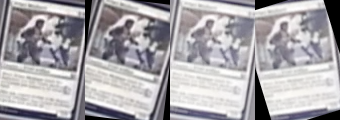
\includegraphics[scale=1.0]{bilder/testSet.png}
    	\caption{Von links nach rechts. Eine Karte aus dem Grunddatensatz. Die gleiche Karte im Rotationsdatensatz, die leicht gedreht wurde. Eine Karte aus dem Helligkeitsdatensatz, die künstlich aufgehellt wurde. Eine Karte aus dem Rotation+Helligkeit Datensatz, die sowohl gedreht als auch aufgehellt wurde.}
    	\label{fig:testSet}
\end{figure}

\subsubsection{Erstellung}

Die Rotation wird durch eine zufällige Drehung um $5°$ - $20°$ umgesetzt. Diese Rotation entspricht etwa der natürlichen Rotation die ensteht, wenn Spieler Karten nicht perfekt waagerecht legen.
Veränderungen in der Beleuchtung werden für jeden Pixel mit folgender Formel berechnet \footnote{\cite[S. 75]{Burg06}}:

\[
I'(x, y) = I(x, y)^\gamma
\]

Der Wert für $\gamma$ wird für jedes Bild zufällig zwischen 0.8 bis 1.8 gewählt. Die starke Tendenz zur Aufhellung anstatt Verdunklung ist dadruch bedründet, dass Spieler oft matte Hüllen um ihre Karten benutzen. Dieser matte Effekt lässt eine Karte deutlich heller erscheinen.
Diese Operationen werden auf jedes Bild im Grunddatensatz angewandt. Dadurch werden jeweils die anderen Datensätze erzeugt.

\subsubsection{Vorverarbeitung}

So wie beim Trainingsdatensatz wird auch für die Testbilder ein Vorverarbeitungsschritt durchgeführt, bevor die Bildmerkmale berechnet werden.
Das Bild wird zuerst auf eine Größe von $70 \times 85$ geschnitten, sodass nur die obere Hälfte der Karte zu sehen ist.
Das Bild wird in ein Graubild umgewandelt und auf eine Größe von $128 \times 128$ skaliert.

\subsection{Klassifikator}
\label{sec:klassifikator}

Im Folgenden wird ein Verfahren vorgestellt, mit dem einer Karte aus dem Testdansatz eine Klasse zugewiesen wird. 

\subsubsection{Idee}

Um einem Testbild eine Klasse zuzuweisen sollen die zuvor bestimmten Merkmale des Trainingsdatensatzes und die Merkmale des Testbildes genutzt werden.
Um diese Merkmale zu finden, werden SIFT, SURF und ORB benutzt.
Die Deskriptoren von SIFT, SURF und ORB sind so konstruiert, dass der gleiche oder ähnliche Bereich in einem Bild einen möglichst gleichen Deskriptorvektor ergibt. 
Dadurch sollten sich die Merkmale im Testbild in den Merkmalen des Trainigsdatensatz wiederfinden lassen.

Es wird der Raum betrachtet, in dem sich alle Vektoren aller Merkmale aus dem Trainingsdatensatz befinden. Nun wird für jedes Merkmal aus dem Testbild jeweils das Merkmal gefunden welches im Merkmalsraum, nach einer festgelegten Distanzfunktion, am nächsten ist.
Im Idealfall würde nun jedes Merkmal aus dem Testbild einem Merkmal der Klasse zugeordnet, zu der es wirklich gehört. Da sich die Trainings- und Testbilder jedoch so stark unterscheiden und die Merkmalsverfahren keine perfekten Ergebnisse liefern, werden einige Merkmale des Testbildes jedoch den falschen Klassen zugeordnet.
Um nun die richtige Klasse zu bestimmen, wird für jede Klasse eine Bewertung erstellt. Die Bewertungsfunktion soll sowohl viele übereinstimmende Merkmale belohnen als auch in Betracht ziehen, wie groß die Distanz zwischen den zugeordneten Merkmalen ist.


\subsubsection{Implementierung}

Im Folgenden wird für SIFT und SURF wird die euklidische Distanz als Distanzfunktionen genutzt. Da der Feature Vektor von ORB binär ist, wird für ORB die Hamming Distanz (siehe \ref{sub:hammingDistanz}) als Distanzfunktion genutzt.

Dadurch, dass jedes Merkmal des Testbildes einem Merkmale im Featureraum zugeordnet wurde, ergibt sich eine Menge $D_i$ für jede Klasse, die die Distanzen zwischen den Merkmalen enthält.
Die Bewertung $s_i$ für die Klasse $i$ wird definiert als: 

\[
s_i = \sum_{d \in D_i} \frac{1}{d^2}
\]

Die Bewertungsfunktion ist so gewählt, dass hohe Distanzen zwischen den Merkmalen weniger zu der Bewertung beitragen, als kleine Distanzen. Der Term $d^2$ bestraft große Distanzen, wodurch sehr gute Paare stärker in die Bewertung einfließen.

Nachdem alle Bewertungen $s_i$ berechnet wurden, wird das Testbild als die Karte klassifiziert, welche die höchste Bewertung hat.
Zudem wird aus allen Bewertungen bestimmt, wie sicher der Klassifikator ist, dass das Testbild richtig klassifiziert wurde.
Hierfür wird die sogenannte Softmax Funktion genutzt \footnote{\cite{Bishop:2006:PRM:1162264}}. Die Funktion nimmt einen Vektor an Werten und beschränkt alle Werte des Vektors in den Bereich [0, 1], sodas die Summe aller dieser neuen Werte 1 ist. Die Softmax Funktion ist definiert als:

\[
f_i(s) = \frac{e^{s_i}}{\sum_j e^j}
\]



\subsection{Durchführung}
\label{sub:durchführung}

Um die Erkennungsrate der verschiedenen Verfahren bewerten zu können, werden diese mit dem oben beschriebenen Klassifikator und den Testdatensätzen getestet.
Hierbei werden jeweils für SIFT, SURF und ORB die vier Testdatensätze durchlaufen und mit dem Klassifikator den Testbildern Klassen zugewiesen. 
Es wird festgehalten, welche Klasse den Testbildern mit welchem Softmaxwert zugewiesen wurde und ob diese Klasse die richige Klasse ist.
Desweiteren wird für jedes Verfahren gemessen, wie lange benötigt wird, um die Merkmale für die Testdaten zu bilden und diese zu klassifizieren. 
So kann im Weiteren ggf. eine Abwägung zwischen Geschwindigkeit und Erkennungsrate der Verfahren getroffen werden.

Die Ergebnisse werden in \ref{sec:auswertung} vorgestellt und ausgewertet.


\section{Auswertung}\raggedbottom 
\label{sec:auswertung}

\subsection{Statistische Auswertung}

\subsubsection{Erkennungsrate}
\label{sub:erkennungsrate}

Ein wichtiger Faktor, um Karten in Videos zu erkennen, ist wie verlässlich ein Verfahren die Karten erkennt. Die Ergebnisse der in \ref{sub:durchführung} besprochenen Durchführung finden sich in Tabelle \ref{table:result} wieder.

\begin{table}
\centering
	\begin{tabular}{  l c c c c  }
	  Verfahren & Normal & Rotation & Helligkeit & Rotation+Helligkeit \\
	  \midrule
	  SIFT & 299 (99.67\%) & 2861 (95.37\%) & 2990 (99.67\%) & 2845 (94.82\%) \\
	  SURF & 295 (98.33\%) & 2925 (97.50\%) & 2964 (98.80\%) & 2940 (98.00\%) \\ 
	  ORB & 298  (99.33\%) & 2930 (97.67\%) & 2952 (98.40\%) & 2925 (97.50\%) \\
	\end{tabular}

\caption{Erkannte Karten pro Verfahren und Datensatz. In Klammern ist jeweils die prozentuale Erkennungsrate angegeben.}
\label{table:result}
\end{table}

Es lässt sich sehen, dass alle Verfahren für den normalen Datensatz eine gute Erkennungrate haben.
Es fällt auf, dass bei Rotation alle Verfahren schlechtere Ergebnisse liefern. Jedoch verliert SIFT am meisten Genauigkeit. Es verliert 5.1\% im Gegensatz zu SURF (1.1\%) und ORB (1.7\%).

Die Softmaxwerte für alle richtig klassifizierten Karten sind bei allen Verfahren relativ hoch (siehe Abbildung \ref{fig:hist}). Die Mittelwerte der Softmaxwerte sind für SIFT 82.01\%, für SURF 94.69\% und für ORB 95.42\%.
Der Durchscnitt der Softmaxwerte für falsch klassifizierte Karten ist für SIFT 0.80\%, für SURF 8.31\% und für ORB 9.71\%. 


\begin{figure}
\begin{subfigure}{.5\textwidth}
  \centering
  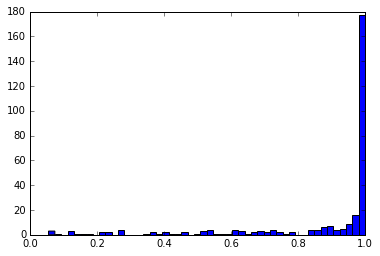
\includegraphics[width=.8\linewidth]{bilder/confidenceSift.png}
  \caption{SIFT}
  \label{fig:sfig1}
\end{subfigure}%
\begin{subfigure}{.5\textwidth}
  \centering
  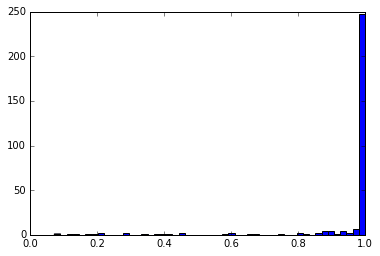
\includegraphics[width=.8\linewidth]{bilder/confidenceSurf.png}
  \caption{SURF}
  \label{fig:sfig2}
\end{subfigure}
\begin{subfigure}{.5\textwidth}
  \centering
  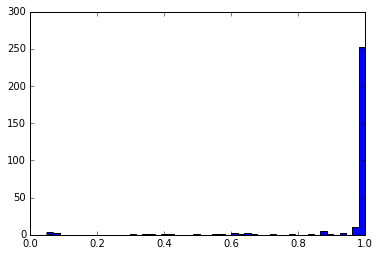
\includegraphics[width=.8\linewidth]{bilder/confidenceOrb.png}
  \caption{ORB}
  \label{fig:sfig2}
\end{subfigure}
\caption{Die Histogramme der Softmaxwerte für richtig klassifizierte Karten.}
\label{fig:hist}
\end{figure}

\subsubsection{Geschwindigkeit}

Damit ein Verfahren zur Erkennung von Karten in einem Video in Echtzeit genutzt werden kann, ist auch die Geschwindigkeit des Verfahrens relevant.
Um diese zu bestimmen, wurde die Laufzeit für die drei Verfahren gemessen. Hierbei wurde nur die Zeit gemessen, die benötigt wird, um eine Karte zu klassifizieren. Die Zeit, die benötigt wird um die Features des Trainigsdatensatzes zu berechnen, wurde nicht beachtet, da dies nur einmal gemacht werden muss, bevor die Karten klassifiziert werden.
Die Ergebnisse dieser Messung finden sich in Tabelle \ref{table:speedResult} wieder.

\begin{table}
\centering
	\begin{tabular}{  l c c   }
	  Verfahren & Zeit gesamt & Zeit pro Karte \\
	  \midrule
	  SIFT & 709s & 2.3s\\
	  SURF & 171s & 0.57s\\ 
	  ORB & 45s & 0.15s \\
	\end{tabular}

\caption{Laufzeit der einzelnen Verfahren für den Standard Datensatz in Sekunden.}
\label{table:speedResult}
\end{table}



\subsection{Bewertung der Ergebnisse}

\subsubsection{Erkennungsrate}

Die Erkennungsrate aller Verfahren ist so hoch, dass sie für den Einsatz in einem Programm zur Liveerkennung von Karten verwendet werden könnten.
Es fällt auf, dass SIFT im Gegensatz zu den anderen Verfahren am stärksten von Rotation der Karten beeinflusst ist. Dies ist erstmal überraschend, da alle Verfahren so konstruiert sind, dass die Merkmale rotationsinvariant sind.
Bei genauerer Betrachtung dieses Sachverhalts fällt auf, dass SIFT für die falsch klassfizierten rotierten Bilder viel mehr Keypoints findet, als SURF und ORB. 
Diese liegen zu einem großen Teil am Rand der Karte und nicht mehr im Bereich, wo das Kartenbild ist (siehe Abbildung \ref{fig:keypointsRot}).
Diese Keypoints und die dazugehörigen Merkmale geben keine Information über das eigentliche Aussehen der Karte.

\begin{figure}[h]
    \centering
		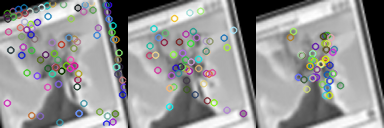
\includegraphics[scale=0.8]{bilder/keypointsRot.png}
    	\caption{Die gefundenen Keypoints sind jeweils mit farbigen Kreisen markiert. Von links nach rechts SIFT, SURF, ORB}
\label{fig:keypointsRot}
\end{figure}


Es ist insbesondere zu beobachten, das alle diese Keypoints an einer Kante liegen.
Dies lässt den Schluss zu, dass SIFT in Bildern mit kleinen Auflösungen ($128 \times 128$ Pixel), häufig Keypoints an Kanten findet, anstatt nur an Ecken.


\subsubsection{Geschwindigkeit}

In der Geschwindigkeit der Verfahren lässt sich ein klarer Unterschied erkennen. Dieser ist allerdings auch zu erwarten. SURF wurde mit dem Ziel entworfen, schneller als SIFT zu sein. Das gleiche gilt für ORB, welches in seinem Paper \footnote{\cite{Rublee:2011:OEA:2355573.2356268}} als effizientere Alternative zu SIFT und SURF vorgestellt wurde.

Damit die Klassifikation in einem Video für einen Anwender nutzbar ist, muss diese ohne große Verzögerung ausgeführt werden können. Mit 2.3 Sekunden ist SIFT eindeutig zu langsam, um zur Klassifikation genutzt zu werden. 
Auch SURF ist mit über einer halben Sekunde Verzögerung fast viermal so langsam wie ORB.
Ein großer Teil des Geschwindigkeitsvorteils von ORB lässt sich damit begründen, dass die von ORB bestimmten Merkmalsdeskriptoren binär sind. Die Berechnung der Hamming Distanz ist deutlich effizienter, als eine Berechnung der euklidischen Distanz.


\section{Erweiterung des Trainingsdatensatzes}\raggedbottom 

Die Erkennungsraten, die in \ref{sec:auswertung} vorgestellt wurden, sind bereits relativ hoch. Dies wurde mit einem Trainingsdatensatz erreicht, der für jede Klasse nur ein einziges Beispiel hatte. Es soll geprüft werden, ob ein größerer Trainingsdatensatz, der mehr Bilder für die Klassen hat, zu einer besseren Erkennungsrate führt. 

Der Trainingsdatensatz soll durch ein automatisiertes Verfahren vergrößert werden. Hierbei sollen automatisch in Videos Bildausschnitte mit Karten gefunden und klassifiziert werden. Die so klassifizierten Bildausschnitte werden mit der gefundenen Klasse zusammen gespeichert und dem Trainingsdatensatz hinzugefügt.


\subsection{Karten Finden}
\label{sec:kartenFinden}

Das folgende Verfahren soll in der Lage sein, in einem Videobild die gezeigten Karten zu finden.
Hierbei wird sich darauf beschränkt, dass Karten, die teilweise überdeckt sind, nicht gefunden werden.
Das Bild wird in einem Vorverarbeitungsschritt so bearbeitet, dass die Ränder der Karten klar abgehoben erkennbar sind. Auf diesem Bild wird dann nach Konturen gesucht, die denen einer Karte entsprechen.

Die Videobilder sind Farbbilder mit einer Auflösung von $1920 \times 1080$ Pixeln.
Das Verfahren wird anhand des Bildes in Abbildung \ref{fig:findCardsSample} veranschaulicht.

\begin{figure}[h]
    \centering
		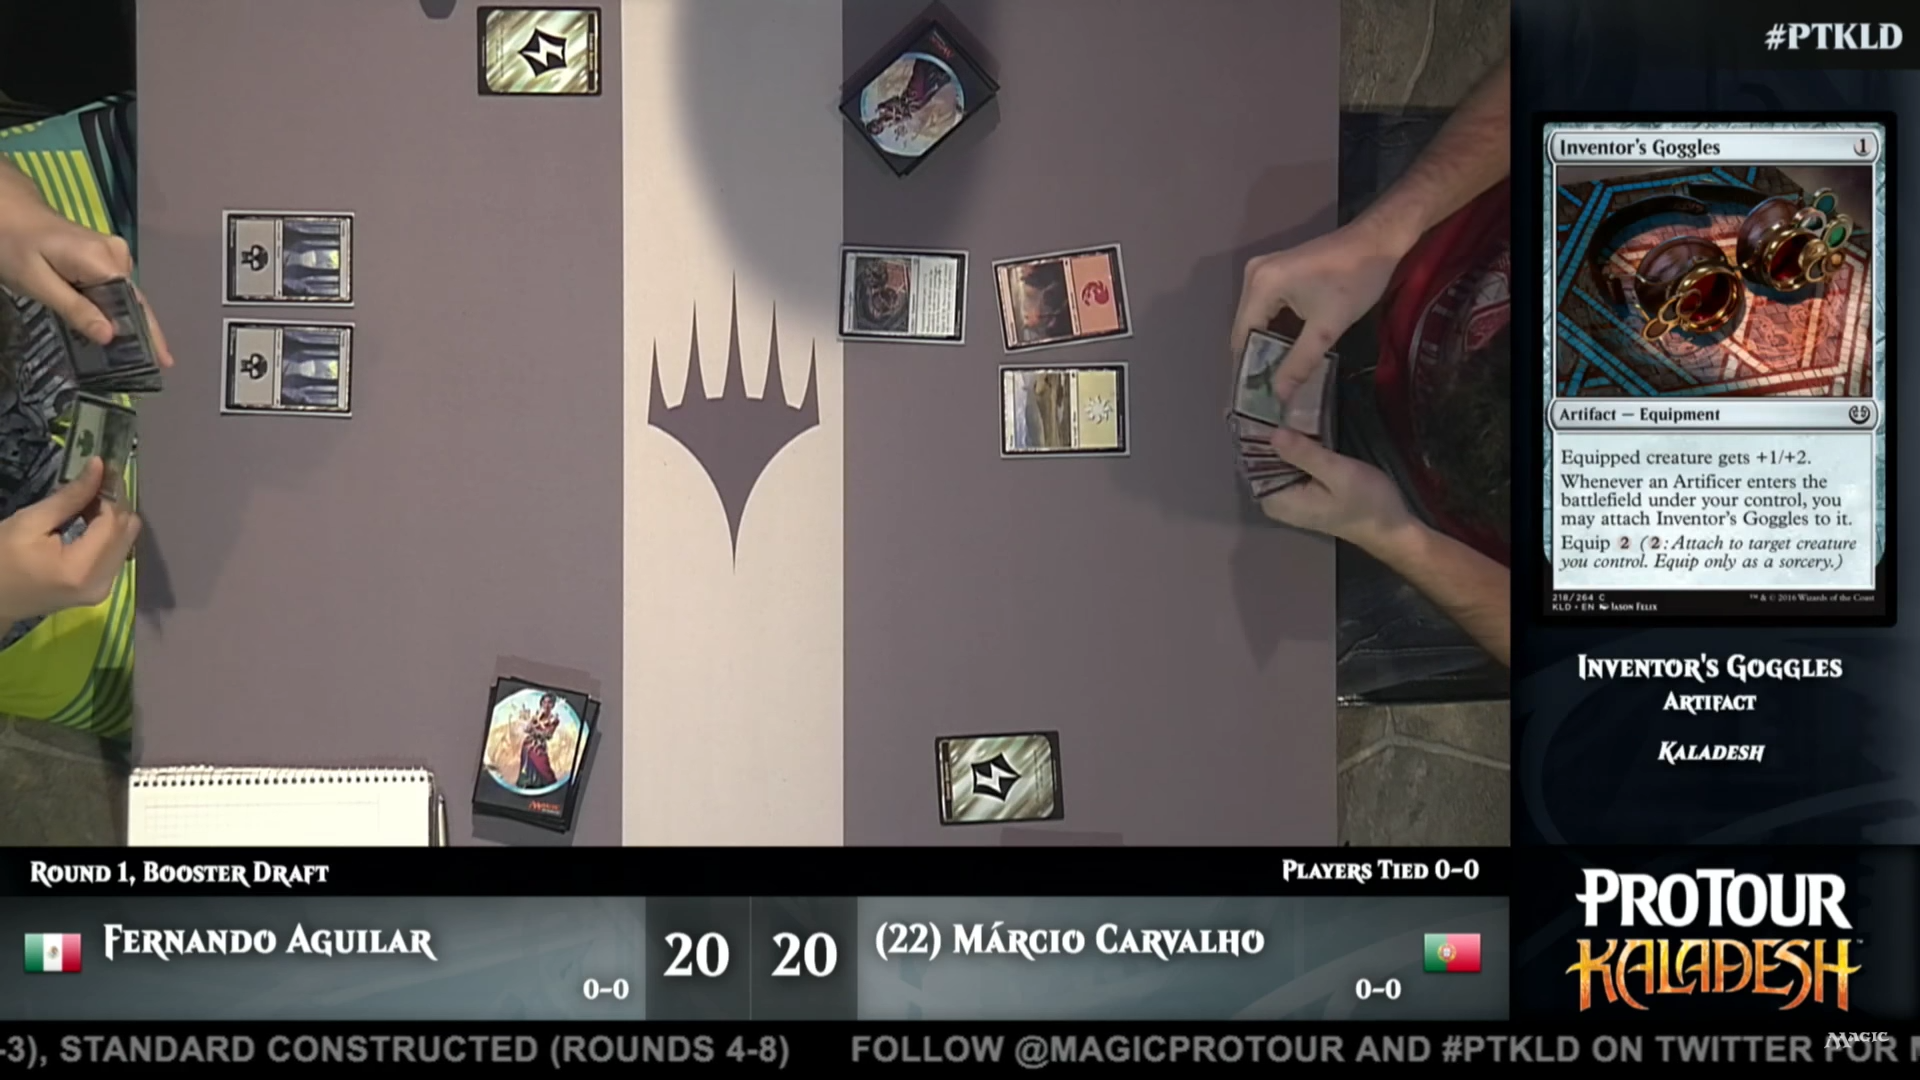
\includegraphics[scale=0.1]{bilder/findCardsSample.png}
    	\caption{Ein Bild aus den Videobildern. Der größte Bereich ist die Aufnahme des Spielbereiches. Rechts daneben befinden sich Informationen zu dem laufenden Turnier. Unterhalb der Spielaufnahme sind Informationen zu den Spielern eingeblendet. }
\label{fig:findCardsSample}
\end{figure}

\subsubsection{Vorverarbeitung}

Bevor in dem Videobild nach Karten gesucht wird, wird das Bild erstmal vorverarbeitet. 
Das Videobild enthält, neben der Aufnahme des Spielbereiches, noch weitere Bereiche mit Informationen für den Zuschauer (siehe Abbildung \ref{fig:findCardsSample}). Um die Karten zu finden, ist nur die Kameraaufnahme des Spielbereiches interessant.
Um nur diesen Bereich zu betrachten, wird das Bild entsprechend zugeschnittten. Das so enstehende Bild (siehe Abbildung \ref{fig:findCardsPreCut}) hat nur noch eine Größe von $1200 \times 845$ Pixeln.


\begin{figure}[h]
    \centering
		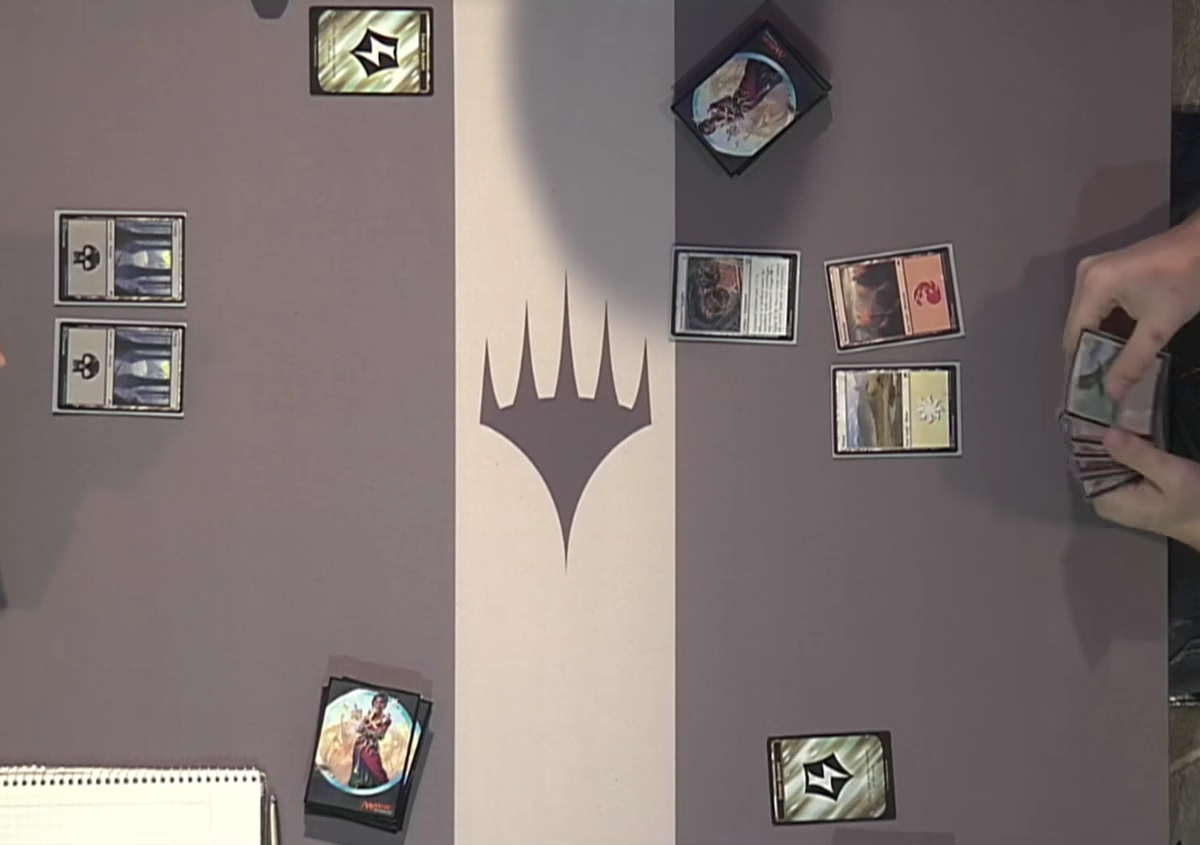
\includegraphics[scale=0.2]{bilder/findCardsPreCut.png}
    	\caption{Das zugeschnittene Bild, sodass nur noch der Spielbereich zu sehen ist.}
\label{fig:findCardsPreCut}
\end{figure}

Damit die Karten in einem späteren Schritt lokalisiert werden könnnen, sollen die Ränder der Karten sichtbar gemacht werden. Dabei kann genutzt werden, dass alle Karten einen schwarzen Rand besitzen.
Das Bild wird zuerst in ein Graubild überführt. In einem Graubild haben schwarze Punkte eine geringe Intensität. Auf diesem Graubild werden alle Pixel, deren Intensität unter einem Schwellwert $t$ liegen, auf den Wert 255 (weiß) gesetzt. Alle Pixel, deren Intensität über dem Schwellwert liegen, werden auf den Wert 0 (schwarz) gesetzt. Das Ergebnis für das Beispielbild kann in Abbildung \ref{fig:findCardsPre} gesehen werden. 
Der Schwellwert wurde experimentell auf $t = 75$ festgelegt.
\begin{figure}[h]
    \centering
		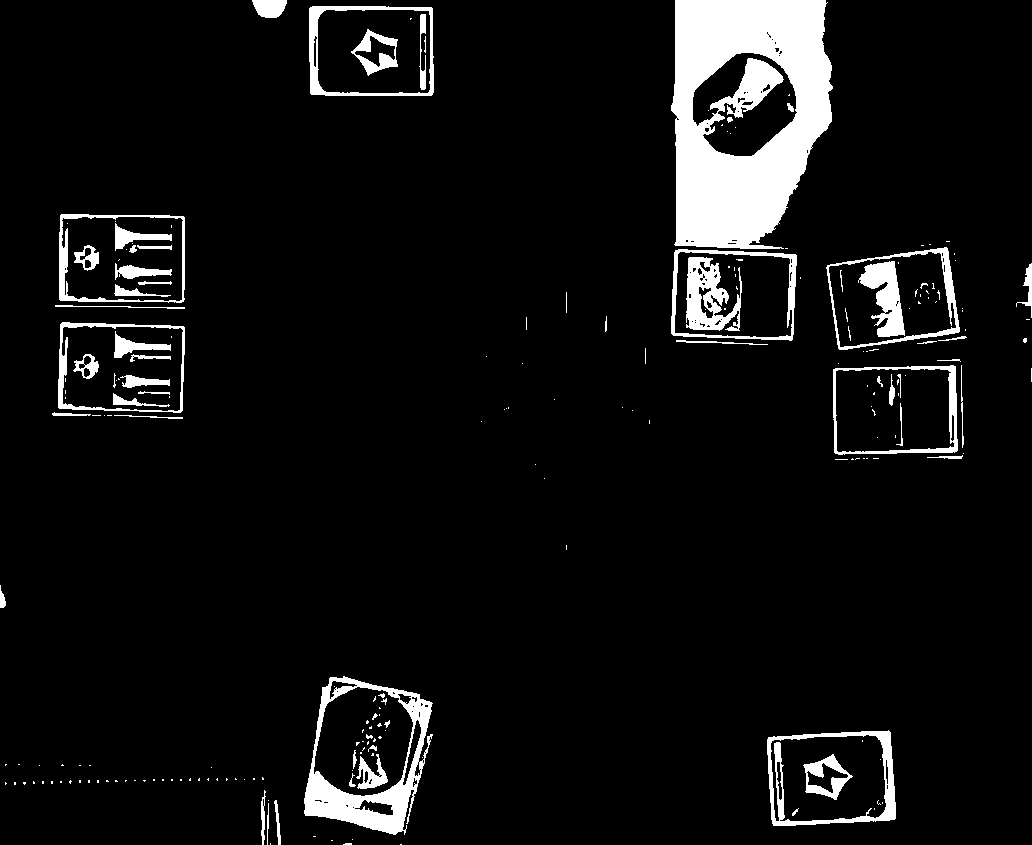
\includegraphics[scale=0.2]{bilder/findCardsPre.png}
    	\caption{Das vorverarbeitete Bild. Die schwarzen Ränder der Karten sind klar erkennbar.}
\label{fig:findCardsPre}
\end{figure}

\subsubsection{Konturerkennung}

Nachdem in der Vorverarbeitung die Ränder der Karten hervorgehoben wurden, sollen nun Konturen erkannt werden, die einer Karte entsprechen.
Zur Konturerkennung wird das von Satoshi Suzuki und Keiichi Abe in ''Topological Structural Analysis of Digitized Binary
Images by Border Following '' \footnote{\cite{journals/cvgip/SuzukiA85}} vorgestellte Verfahren genutzt.

Das Verfahren liefert für jede gefundene Kontur eine Liste an miteinander verbundenen Randpunkten dieser Kontur. Um besser mit der Kontur umgehen zu können, soll die große Liste an Randpunkten reduziert werden. 
Hierfür wird die Kontur mit dem Douglas-Peucker-Algorithmus (siehe \ref{sec:douglas}) approximiert.


\begin{figure}[h]
    \centering
		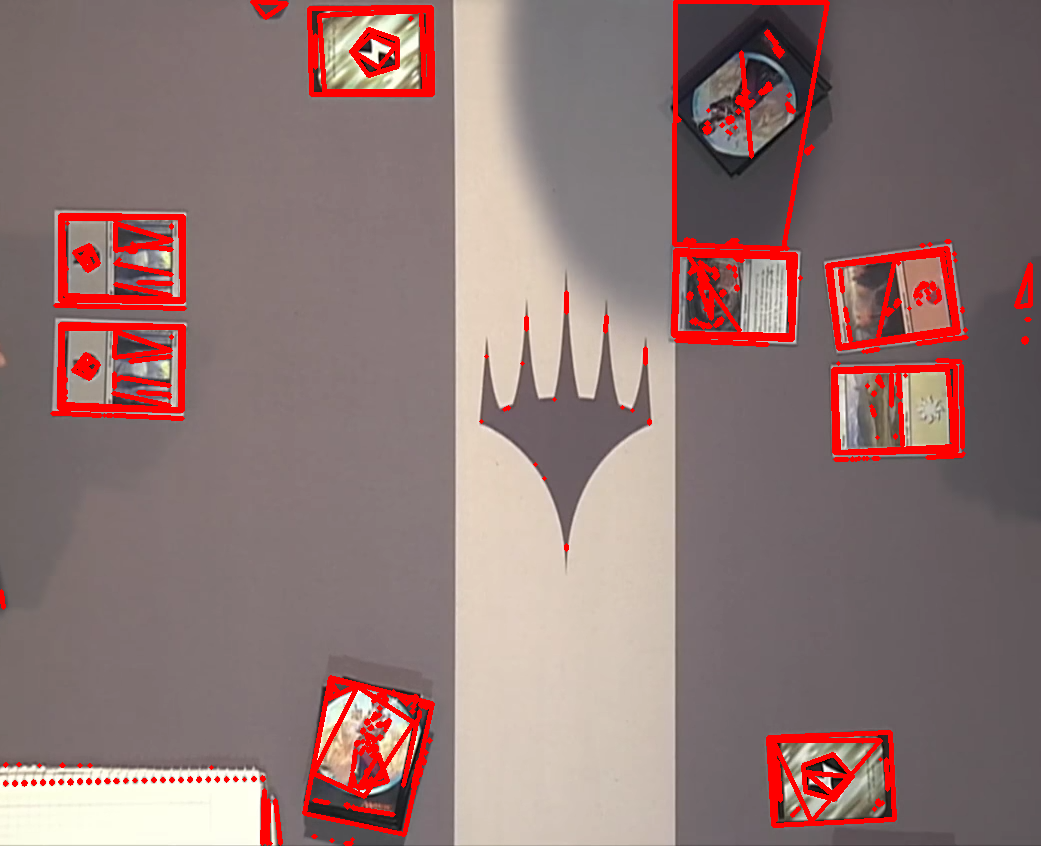
\includegraphics[scale=0.2]{bilder/findCardsContour.png}
    	\caption{Die im vorverarbeiteten Bild gefundenen Konturen sind jeweils rot umrandet.}
\label{fig:findCardsContour}
\end{figure}

Die approximierten Konturen sind in Abbildung \ref{fig:findCardsContour} zu sehen. Ein großer Teil der gefundenen Konturen sind keine Karten. Aus allen gefundenen Konturen sollen die herausgefiltert werden, die keine Karten sind.
Eine Kontur, die zu einer Karte gehört, besteht nach der Approximation nur noch aus vier Randpunkten. Zudem liegt die Größe der Fläche, die diese Kontur einschließt, in einer gewissen Spanne, da alle Karten gleich groß sind.
Aus allen gefunden Konturen werden die gefiltert, die nicht aus vier Punkten bestehen und deren eingeschlossene Fläche kleiner als 5000 und größer als 15000 Pixel ist. Die Grenzen für die Flächen wurden experimentell bestimmt.


Die übrig bleibenden Konturen sind in Abbildung \ref{fig:findCardsFinal} dargestellt.
Die Bildausschnitte in diesen Konturen dienen später als Eingabe für den Klassifikator.

\begin{figure}[h]
    \centering
		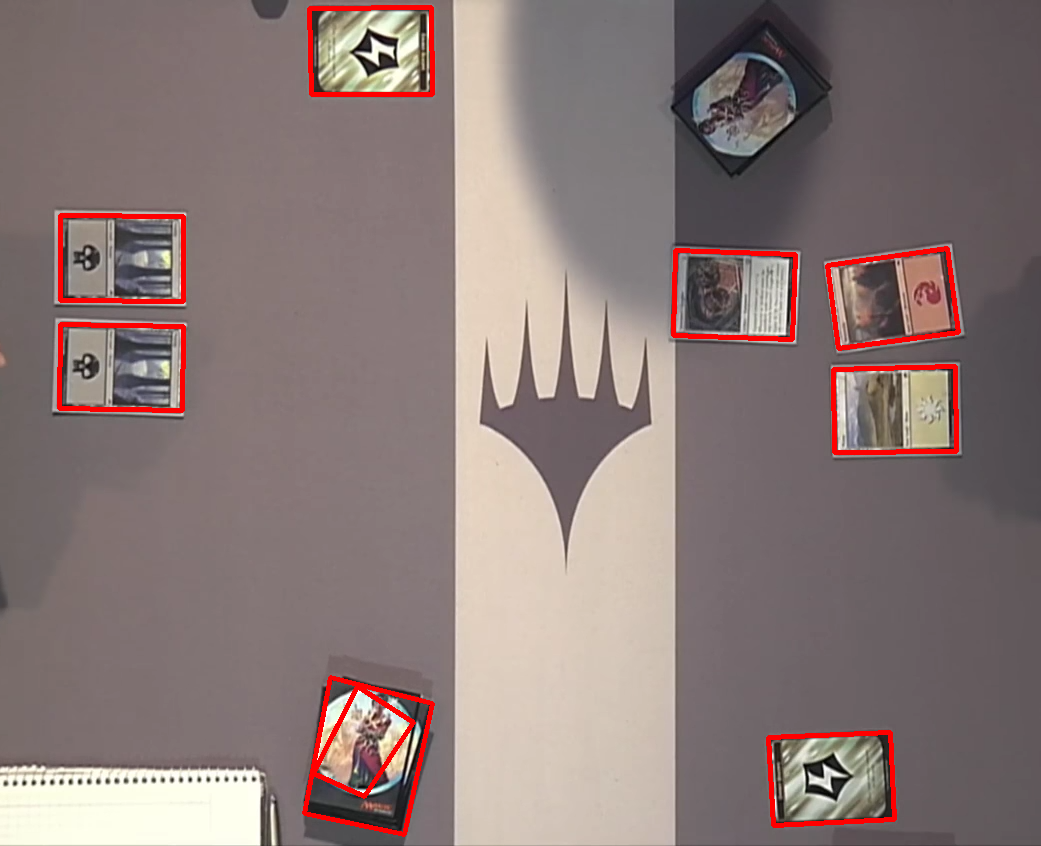
\includegraphics[scale=0.2]{bilder/findCardsfinal.png}
    	\caption{Alle Konturen, die nicht gefiltert wurden.}
\label{fig:findCardsFinal}
\end{figure}


\subsection{Erweiterung des Trainingsdatensatzes}

Mit dem in \ref{sec:kartenFinden} gezeigten Verfahren zur Lokalisierung von Karten und dem Klassifikator soll der Trainingsdatensatz erweitert werden.

\subsubsection{Idee}

Mit einer Kombination aus Lokalisierung und Klassifikation können Karten automatisch aus einem Video herausgeschnitten und klassifiziert werden.
Das Video wird durchlaufen und in regelmäßigen Abständen wird in dem Videobild nach Karten gesucht. Sobald die Karten lokalisiert wurden, werden diese automatisiert, anhand der gefundenen rechteckigen Kontur, ausgeschnitten. 
Diese Bildausschnitte werden mit dem in \ref{sec:klassifikator} beschriebenen Klassifikator klassifiziert. Es soll vermieden werden, dass falsch klassifizierte Karten in den erweiterten Trainingsdatensatz aufgenommen werden. Um dies zu verhindern, wird eine so klassifizierte Karte nur in den erweiterten Trainingsdatensatz aufgenommen, wenn ihr Softmax Wert über einer bestimmten Schwelle liegt.

Als Trainingsvideos werden die Videos in der YouTube Playlist \url{https://www.youtube.com/playlist?list=PLyUK7d88voIirGp0IbtppzOAuMVC4ZVcW} genutzt.

\subsubsection{Implementierung}

Jedes der Videos wird einmal komplett durchlaufen. Da zwischen aufeinanderfolgenden Videobildern kein großer Unterschied besteht, wird nicht jedes einzelne Bild betrachtet.
Es wird nur jedes 180te Videobild betrachtet. Da die Videos 30 Bilder pro Sekunde haben, entspricht das einer Wartezeit von 6 Sekunden.
Bei jedem betrachtetem Bild werden zuerst Bildausschnitte mit dem in \ref{sec:kartenFinden} beschriebenen Verfahren gefunden. 

Die gefundenen Bildausschnitte werden mit dem Klassifikator klassifiziert.
Der Klassifikator wird hierbei mit ORB verwendet. Die Wahl für ORB ist daduruch begründet, dass es das schnellste Verfahren ist und eine gute Erkennungsrate hat (siehe \ref{sec:auswertung}).

Um falsche Klassifikationen nicht mit in den erweiterten Testdatensatz aufzunehmen, wird der Softmax Wert für die Klassifikation betrachtet. Liegt dieser über einer Schwelle $t = 0.8$, so wird die ausgeschnittene Karte als Bild mit der gefundenen Klasse gespeichert. Der Wert von $t = 0.8$ wird gewählt, da in Abbildung \ref{fig:hist} beobachtet wurde, dass fast alle Softmax Werte richtig klassifizierter Karten über 80\% liegen. So werden fast alle richtig klassifizierten Karten über dem Schwelllwert liegen und jede falsch klassifizierte unter ihm.



\subsection{Auswertung}

Der Trainingsdatensatz wurde mit dem in \ref{sec:kartenFinden} erläuterten Verfahren erweitert. Dieser Trainingsdatensatz enthält neben den ürsprünglichen 264 Bildern, 1320 Bilder verteilt auf 129 Klassen.

Bei dieser Auswertung wird nur noch das Verfahren ORB betrachtet, da die beiden anderen Verfahren aufgrund ihrer Geschwindikeit nicht für eine Erkennung in Echtzeit nutzbar sind.

\subsubsection{Erkennungsrate}

Nachdem der Trainingsdatensatz erweitert wurde, lassen sich Veränderungen in der Erkennungsrate beobachten.
Während die Erkennung beim Standarddatensatz leicht schlechter wurde, ist die Erkennungsrate für die drei anderen Datensätze gestiegen (siehe Abbildung \ref{table:result2}).
Es ist zu beobachten dass es für alle 129 Klassen die mehr Trainigsdaten erhalten haben keine falsch klassfizierte Karte mehr gibt. Alle falsch klassifizierten Karten stammen aus den 135 Klassen, für die keine Trainigsdaten aus Videos generiert wurde.
Dies wirft die Vermutung auf, dass mehr Trainingsvideos in denen alle Klassen gefunden werden können, zu einem noch besseren Ergebnis führe könnten.

\begin{table}
\centering
	\begin{tabular}{  l c c c c  }
	  Verfahren & Normal & Rotation & Helligkeit & Rotation+Helligkeit \\
	  \midrule
	  ORB & 297  (99.00\%) & 2944 (98.13\%) & 2954 (98.47\%) & 2938 (97.93\%) \\
	\end{tabular}

\caption{Erkannte Karten nachdem der Trainingsdatensatz erweitert wurde. In Klammern ist jeweils die prozentuale Erkennungsrate angegeben.}
\label{table:result2}
\end{table}


\subsubsection{Geschwindigkeit}

Durch den größeren Trainigsdatensatz gibt es mehr Merkmale, für den Merkmalsabgleich. Dadurch verlängert sich die Zeit, die gebraucht wird um eine Karte zu klassifizieren.
Es wurden 54 Sekunden gebraucht um den ganzen Standarddatensatz zu klassifizieren. Dies entspricht ca. 0.19 Sekunden pro Karte.
Diese Geschwindigkeit ist immernpch ausreichend um Karten in Echtzeit zu klassifizieren.

\section{Fazit}\raggedbottom 

Diese Arbeit wurde mit dem Ziel begonnen, ''Magic the Gathering'' Karten in Videobildern zu finden und zu erkennen, um eine Grundlage für eine Anwendung zu schaffen, die dies automatisch in einem Livevideo kann. 

Zur Klassifizierung von Karten werden Bildmerkmale genutzt. Insbesondere wurde die Anwendbarkeit von SIFT, SURF und ORB analysiert.
Bei den drei untersuchten Verfahren zeigt sich, dass alle in der Lage sind, Karten mit einer hohen Erkennungsrate zu klassifizieren. Alle Verfahren konnten eine Erkennnungsrate von über 98\% erreichen.

Dabei zeigte sich ein Performance Abfall des SIFT Verfahrens bei gedrehten Karten. Dieser konnte bei einer näheren Anaylse auf eine Hohe Anzahl von Keypoints an Kanten zurück geführt werden. 

Aufgrund der langsamen Geschwindigkeit von SIFT und SURF eignet sich nur ORB dafür, genutzt zu werden, um eine Anwendung zu Implementieren, die Karten in Echtzeit erkennt.

Es konnte eine grundlegende Methode zur Lokalisierung von Karten in Videobildern entwickelt werden. Diese Methode ist jedoch nicht in der Lage, teilweise verdeckte Karten zu finden. Zudem muss weitergehend untersucht werden, wie gut die Methode Karten lokalisiert.

Durch die Kombination der Lokaliserung und Klassifizierung von Karten, konnte der Trainingsdatensatz mithilfe von bereits vorhandenen Videos automatisch erweitert werden. Diese Erweiterung führte zu einer leichten Verbesserung Erkennungsrate. Es lässt sich jedoch erkennen, dass durch mehr Videomaterial mit mehr verschiedenen Karten sich die Erkennungsrate weiter steigern lässt.

Durch Lokalisierung und Klassifizierung sind die Grundlagen für eine automatische Erkennung von Karten in Echtzeit gelegt. Eine solche Anwendung würde es neuen Spielern des Spiels ermöglichen, Turniere mitzuverfolgen und die Strategien der Spieler nachzuvollziehen.
Um so eine Anwendung zu implementieren, muss geklärt werden, wie sie die Videodaten eines im Browser laufenden Livestreams abrufen kann. 

%%%%%%%%%%%%%%%%%%%%%%%%%%%%%%%%%%%%%%%%%%%%%%%%%%%%%%%%%%%%%%%%%%%%%%%%
%%%% ENDE TEXTTEIL %%%%%%%%%%%%%%%%%%%%%%%%%%%%%%%%%%%%%%%%%%%%%%%%%%%%%
%%%%%%%%%%%%%%%%%%%%%%%%%%%%%%%%%%%%%%%%%%%%%%%%%%%%%%%%%%%%%%%%%%%%%%%%

\clearpage

% Entfernen Sie das Kommentar aus der nachfolgenden Zeile, falls Sie einen Anhang in der Arbeit verwenden wollen. Beachten Sie, dass Sie sich im Verlauf der Arbeit mit \ref{...} (z.B. \ref{anhang:zusatz1}) auf den Anhang beziehen.
%\newpage
\appendix
\section{Anhang}

\subsection*{Zusatzteil 1} \label{anhang:zusatz1}

Dies ist ein Anhang.

\clearpage

\bibliography{references}
\bibliographystyle{alphadin}
%\vspace*{\fill}

\clearpage

\listoffigures

\listoftables

%\pagebreak

%\printindex
\end{document}
